%% msPrettyman_final

\documentclass[%
aip,
% jmp,
% bmf,
% sd,
% rsi,
amsmath,amssymb,
%preprint,%
reprint,%
%author-year,%
%author-numerical,%
% Conference Proceedings
]{revtex4-1}

\draft % marks overfull lines with a black rule on the right

\usepackage{graphicx}% Include figure files
\graphicspath{{figures/}}
\usepackage{dcolumn}% Align table columns on decimal point
\usepackage{bm}% bold math
%\usepackage[mathlines]{lineno}% Enable numbering of text and display math
%\linenumbers\relax % Commence numbering lines

\usepackage[utf8]{inputenc}
\usepackage[T1]{fontenc}
\usepackage{mathptmx}

\newcommand{\x}{{\mathbf x}}
\newcommand{\y}{{\mathbf y}}
\newcommand{\etab}{{\mathbf \eta}}

\usepackage{color}
\newcommand{\noteRed}[1]{{#1}}
%\newcommand{\newNote}[1]{\color{red} {#1}}
\newcommand{\newNote}[1]{{#1}}
\begin{document}
	
	\preprint{AIP/123-QED}
	
	\title[Generalised early warning signal methods]{Generalised early warning signals in multivariate and gridded data with an application to tropical cyclones}
	% Force line breaks with \\
	
	\author{J. Prettyman}
	\altaffiliation[Also at ]{National Physical Laboratory}%Lines break automatically or can be forced with \\
	\author{T. Kuna}%
	\affiliation{ 
		University of Reading, Whiteknights, Reading, RG6 6AX, UK%\\This line break forced with \textbackslash\textbackslash
	}%	
	\author{V. Livina}
	\affiliation{%
		National Physical Laboratory, Hampton road, Teddington, TW11 0LW, UK%\\This line break forced% with \\
	}%
	\email{Correspondence to v.livina@npl.co.uk}
	
	\date{\today}% It is always \today, today,
	%  but any date may be explicitly specified







\begin{abstract}
Tipping events in dynamical systems have been studied across many applications, often by measuring changes in variance or autocorrelation in a one-dimensional time series. In this paper, methods for detecting early warning signals of tipping events in multi-dimensional systems are reviewed and expanded. An analytical justification of the use of dimension-reduction by empirical orthogonal functions, in the context of early warning signals, is provided and the one-dimensional techniques are also extended to spatially separated time series over a 2D field. The challenge of predicting an approaching tropical cyclone by a tipping-point analysis of the sea-level pressure series is used as the primary example, and an analytical model of a moving cyclone is also developed in order to test predictions. We show that the one-dimensional power spectrum indicator may be used following dimension-reduction, or over a 2D field. We also show the validity of our moving cyclone model with respect to tipping-point indicators.
\end{abstract}

\pacs{}

\maketitle

\begin{quotation}
	Many dynamical systems experience sudden shifts in behaviour, often referred to as tipping points or critical transitions. A volume of work is dedicated to detecting and predicting these critical transitions, often making use of generic early-warning signal (EWS) indicators based on auto-correlation \cite{held2004,dakos2008} and increasing variance \cite{carpenter2006,scheffer2009}. Similar indicators based on other scaling properties of the time series, namely detrended fluctuation analysis \cite{kantelhardt2001,livina2007} and power spectrum scaling \cite{prettyman2018}, have also been used. Other methods have estimated parameters to fit a model to the data, both for detecting critical transitions \cite{livina2010,livina2011,lenton2012} and for predicting future transitions dynamics \cite{livina2013,kwasniok2018}.
\end{quotation}

\section{Introduction}
\label{sec:Intro}

Early warning signal techniques generally are applied only to univariate data, often one-dimensional time series from a single data source or model output. In an effort to study multidimensional geophysical variables we here consider cases where we have more than one time series, either because there is more than one measured variable, or because a variable is measured at several locations, or both of these simultaneously. In the first case it may suffice to attempt an EWS detection on each time series individually, but one can envision a scenario where it is not possible to detect an EWS in $X(t)$ nor $Y(t)$ but, considered together in some way, an EWS is visible. It may therefore be worthwhile to investigate the possibility of a two (or more) dimensional analogue to existing one-dimensional techniques. In the case of gridded data it is common to use Empirical Orthogonal Functions (EOF), also known as Principal Component Analysis (PCA), to reduce the dimensionality \cite{vonstorch,jolliffe1986}, this technique has also been more specifically applied to EWS methods \cite{held2004,bathiany2013part1,kwasniok2018}.

There has been a large amount of work involving the use of multiple data sources spread over a geographic area, such as complex network analysis in climate \cite{tsonis2006,yamasaki2008,gozolchiani2011} which has been applied to the El Ni{\~n}o. In Refs.~\onlinecite{ludescher2013,ludescher2014} the cross-covariance is calculated between points on a grid inside a region of interest (in this case, the El Ni\~{n}o basin) and points outside, in contrast with the EOF method which considers the  covariance of all available points. Principal interaction and oscillation patterns (PIPs and POPs) can be considered as extensions of the EOF method and provide additional techniques for the dimension reduction of complex systems \cite{hasselmann1988}.

In Sec.~\ref{sec:1DTropicalCyclone} we review previous one-dimensional EWS research, and then we review and analyse methods which may be used to calculate an EWS with an input of two variables, namely the use of EOFs for dimension-reduction (in Sec.~\ref{sec:EOF}), and the methods presented in Ref.~\onlinecite{williamson2015} (in Sec.~\ref{sec:Williamson}). In Sec.~\ref{sec:AppliedHurricanes} we use the example of the approaching tropical cyclone as a test case for these methods. In Sec.~\ref{sec:MultipleTimeSeries} we present a method to visualise early warning signals in a dynamical system over a 2D field, and apply this method to time series of variables measured at geographically separated locations in the vicinity of an approaching tropical cyclone. In Sec.~\ref{sec:Model} we present a novel stochastic model of a moving cyclone in order to test the method. 

\section{Early warning signals in tropical cyclone data}
\label{sec:1DTropicalCyclone}

A number of techniques are available to detect an early warning signal (EWS) in a dynamical system given time series data as input \cite{livina2007,scheffer2009,lenton2012}. Many such techniques detect changes in an indicator (variance, autocorrelation or scaling properties) over time by calculating the value of the indicator in a sliding window of $N$ points, where $N$ is typically in the order of 10\% to 50\% of the length of the series.

\begin{figure}
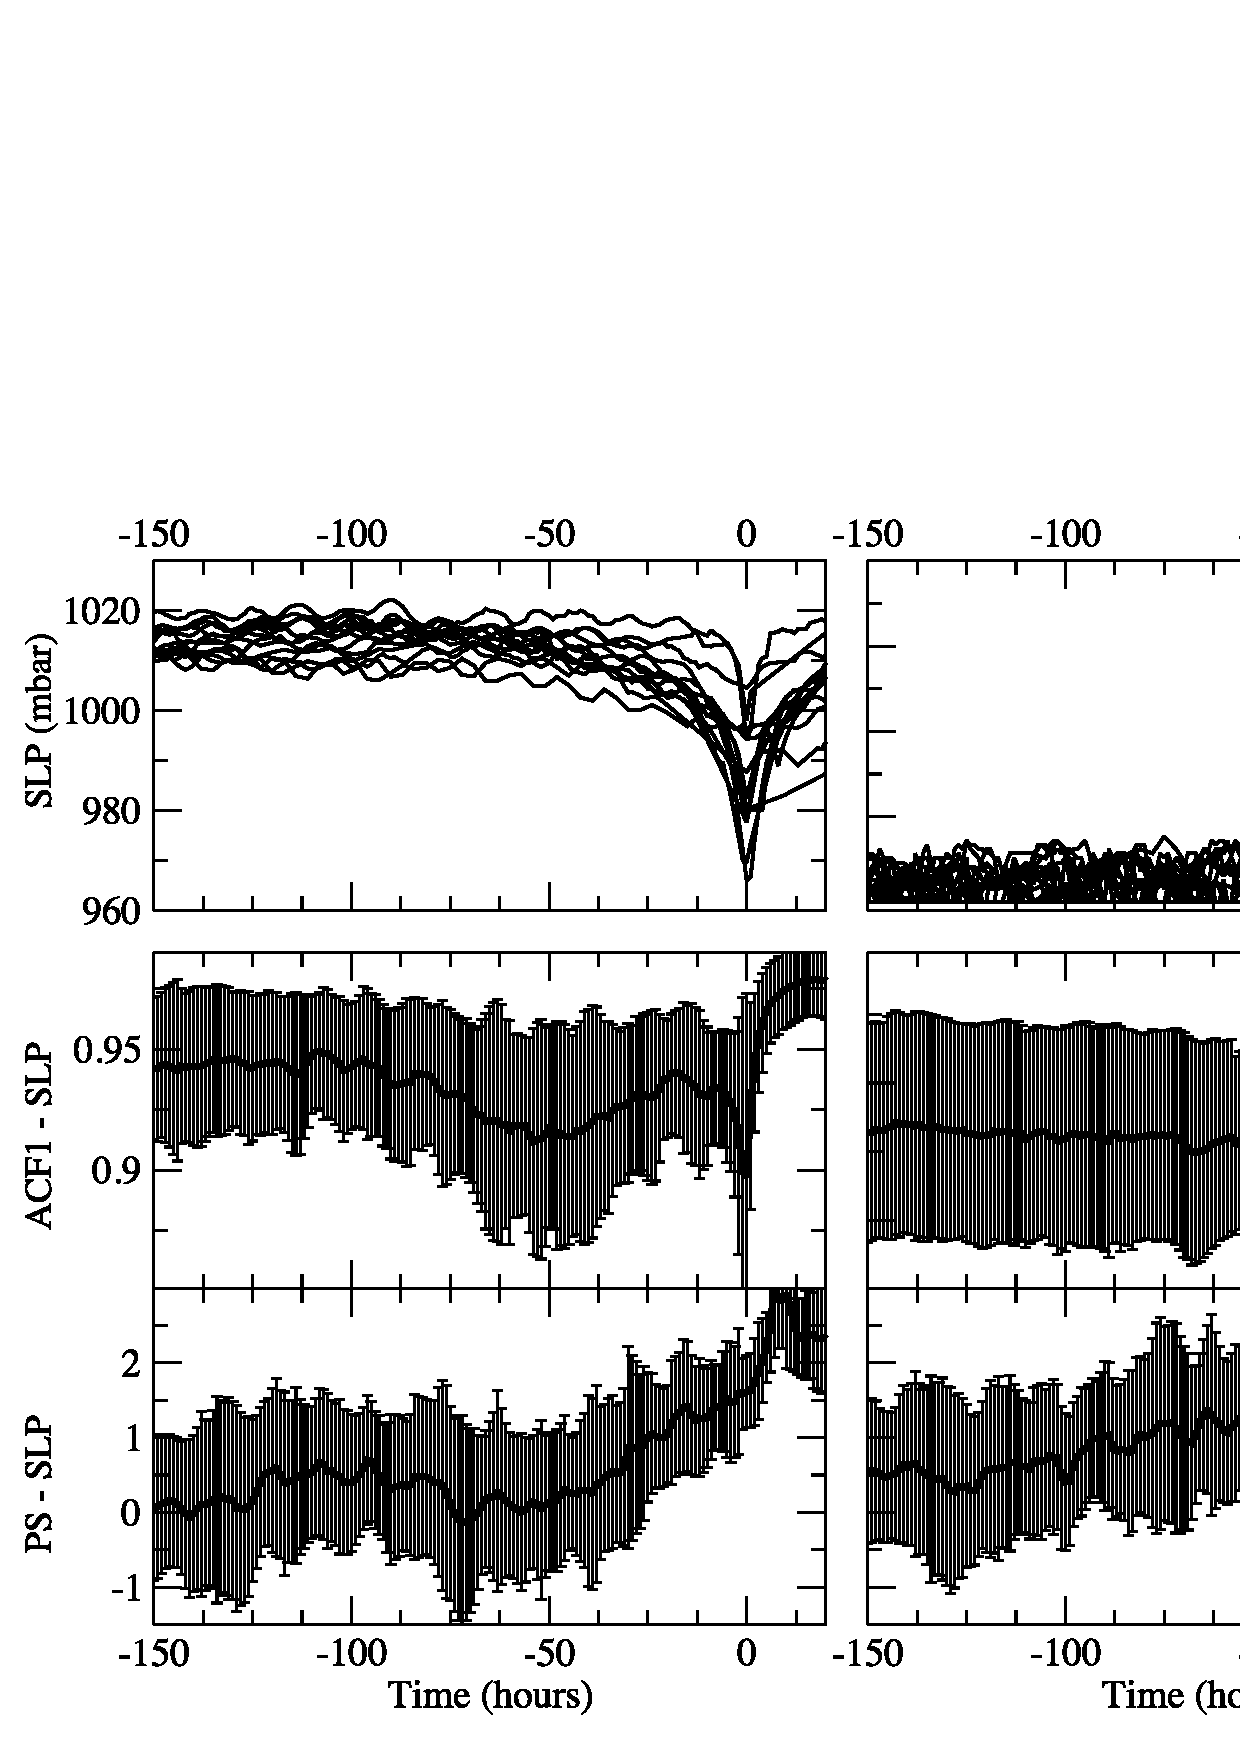
\includegraphics[width = \columnwidth]{01_ACF1andPS}\caption{\label{fig_ACF1andPS} The sea-level pressure (SLP) and wind speed (WS) time series for all fourteen cyclones are shown (top row) with all series centred so that the point of minimum pressure occurs at zero. The mean ACF1 indicator is shown for both variables (middle row). The mean PS indicator is shown for both variables (bottom row). We note that the ACF1 indicator for the SLP variable does not appear to rise before time zero, all other indicators rise to some extent.}
\end{figure}

In Ref.~\onlinecite{prettyman2018} three {\noteRed tipping point} indicators are compared: lag-1 autocorrelation (ACF1), the detrended fluctuation analysis (DFA) exponent, and a novel indicator (PS) based on the scaling exponent of the power spectrum. {\noteRed The ACF1 indicator is obtained by calculating the lag-1 autocorrelation function (ACR) of a time series in a sliding window, the length of which may be determined by a sensitivity analysis (see the supplementary material). The DFA and PS indicators are  obtained similarly, but rather than the lag-1 ACR, either the DFA exponent\cite{kantelhardt2001} or power spectrum scaling exponent $\beta$ is calculated. To obtain $\beta$, the slope of the power spectrum $S(f)$ of the data is estimated and plotted on logarithmic axes\cite{bak1988}, we then have the scaling relationship 
	\begin{equation}
	\label{eqn:1D:PSexponent}
	S(f) \sim f^{-\beta},
	\end{equation} 
where $f$ is the frequency and $S$ is the spectral power. In this study we have calculated the power spectrum scaling exponent using the standard periodogram, obtained from the absolute value of the fast Fourier transform.}

These {\noteRed tipping point indicators} are used to investigate early warning signals in the sea-level pressure time series measured at a fixed point during the approach of a tropical cyclone. In this paper we study the same fourteen tropical cyclones, but extend the scope to a second variable, wind speed. The weather station data is obtained from the HadISD 2017 raw data set \cite{HadISD,HadISD_dunn12,HadISD_dunn14,HadISD_dunn16,HadISD_smith} with no further filtering, and no detrending, applied. The stations are chosen close to the coast, within a radius of 10km of the cyclone's landfall. We use both the sea-level pressure and wind speed data for the purpose of investigating early warning signals in a two-variable system. In Fig.~\ref{fig_ACF1andPS} the time series of both variables are shown (centred on the time of minimum pressure for each cyclone) along with the ACF1 and PS indicators calculated in a window of 100 points (100 hours). We note that the ACF1 indicator provides no early warning signal when applied to the sea-level pressure series, nor a convincing one when applied to the wind speed series. The PS indicator does increase prior to time zero in both cases, the effect is more marked in the sea-level pressure case. Since the two variables give distinct indicator series, it is reasonable to study both, since one may provide information that the other does not. In the following sections we provide detailed analysis of this system.

\section{Empirical Orthogonal Functions}
\label{sec:EOF}

The method of Empirical Orthogonal Functions (EOF) is widely used in geosciences for the purpose of reducing dimensionality \cite{bjornsson1997,shaw2009}. This method has been used \cite{held2004} to reduce the dimensionality of a data set prior to identifying an early warning signal by calculating the ACF1 indicator in the now one-dimensional time series.

The EOF method projects a multidimensional system onto a new basis chosen such that the variance of the new first variable is maximised, and the variance of the second variable is maximal given the choice of the first basis vector, etc.. Here we consider only the projection onto the first basis vector, known as the first loading vector. This maximum-variance, one-dimensional time series typically captures the interesting features of the system, such as large changes in one of the variables. It is not clear, however, that this will capture dynamical features important to the calculation of early warning signals, such as changes over time in variance, autocorrelation or spectral properties. Whilst the EOF method projects a system onto the component with largest variance, what is useful in the study of EWS's is the size of the {\noteRed increment} in variance, autocorrelation, etc., not the size of the variance itself. {\noteRed It is not obvious that the component exhibiting the largest variance increment will be similar to the component with the largest variance.} It is certainly not obvious when considering other indicators such as autocorrelation.

To test the hypothesis that the first EOF score will capture properties important to the calculation of early warning signals, we study the general {\noteRed linear} dynamical system $[\mathbf{x}_n]$ described by
\begin{equation}
\mathbf{x}_{n+1} = B\mathbf{x}_n + S\mathbf{\eta}_n
\label{eqn_discreteSystem}
\end{equation}
where the $\eta_n$ are column vectors with each element independent and from a standard normal distribution. We control the system with the condition that $B$ is contracting, i.e. that all eigenvalues are less than one, in this case {\noteRed the system has zero mean in the long-term.} If we instead say that $B$ is such that, as $n$ increases, the first eigenvalue $\lambda_1$ increases, then we have a system with a bifurcation when $\lambda_1=1$. Clearly, if there is any early warning signal of this bifurcation, it will be most apparent in the one-dimensional basis consisting of the first eigenvector of $B$, since this is where the change in $\lambda_1$, which governs the bifurcation, will be observed. The early warning signal will not be observed in any basis orthogonal to this one. We therefore expect that, if EOF is a useful method to reduce dimensionality prior to detecting an early warning signal, it will project the series $[\mathbf{x}_n]$ onto a first loading vector which does not differ significantly from the first eigenvector of~$B$. 

We calculate the first loading vector according to the EOF method, for the general system given in (\ref{eqn_discreteSystem}), by first finding the covariance matrix given by 
\begin{equation}
C = \mathbb{E}\left[\left(\x_n-\mathbb{E}(\x_n)\right) \left(\x_n-\mathbb{E}(\x_n)\right)^\top\right]
\label{eqn_covarianceMatrix}
\end{equation} 
where we use the empirical mean to estimate the expected value in each case. We also consider the long term limit of the system, that is, we consider $\x_n$ for $N_0\leq n\leq N$ rather than $0\leq n \leq N$, where $N_0$ is chosen to be sufficiently large that $B^{N_0}$ is negligible. In order to evaluate the matrix $C$ we must rewrite (\ref{eqn_discreteSystem}) as an explicit expression for $\mathbf{x}_n$ {\noteRed in terms of $\mathbf{x}_0$:
\begin{align}
\begin{split}
\x_k &= B^k\x_0 + \left[ \sum_{j=0}^{\infty} B^{j} S \etab_{k-j} - \sum_{j=k}^{\infty} B^{j} S \etab_{k-j}\right]\\
&= B^k\x_0 + \left[ \sum_{j=0}^{\infty} B^{j} S \etab_{k-j} - \sum_{j=0}^{\infty} B^{j+k} S \etab_{-j}\right]\\
&= \sum_{j=0}^{\infty} B^{j} S \etab_{k-j} - B^k \left(\sum_{j=0}^{\infty} B^{j} S \etab_{-j} - \x_0\right).
\end{split}
\label{eqn_discreteSystem_rewrite}
\end{align}
We find that} the mean of $\x$ is zero and (\ref{eqn_covarianceMatrix}) is reduced to
\begin{equation}
C = \frac{1}{N-N_0} \sum_{N_0}^{N}\left[\x_n \x_n^\top\right].
\label{eqn_covarianceMatrix_simplified}
\end{equation} 
Here, we use the fact that $\mathbb{E}((\eta_{n-j})(\eta_{n-r})^\top)$ is the identity matrix where $r = s$ and the zero matrix otherwise. We then find that 
\begin{equation}
\mathbb{E}(C) = \sum_{j=0}^\infty B^j S S^\top (B^\top)^j.
\end{equation} 
We now restrict our analysis to the two-dimensional case and we also only consider the case where $B$ is diagonal, which is equivalent to requiring that $B$ is diagonalisable. {\noteRed Since we are interested in the system approaching the bifurcation when the first eigenvalue of $B$ is equal to one, we make the choice that $b_{11}\approx1$ (from below), where $b_{ij}$ and $s_{ij}$ are the elements of $B$ and $S$.} It is then possible to calculate the eigenvectors of $\mathbb{E}(C)$ which we can write in the closed form
\begin{equation}
\mathbb{E}(C) = \left[ 
\begin{array}{cc}
\frac{s_{12}^2+s_{11}^2}{1-b_{11}^2} & \frac{s_{12}s_{22}+s_{11}s_{21}}{1-b_{11}b_{22}}\\
\frac{s_{12}s_{22}+s_{11}s_{21}}{1-b_{11}b_{22}} & \frac{s_{22}^2+s_{21}^2}{1-b_{22}^2}
\end{array}
\right].
\label{eqn_matrixD}
\end{equation}
{\noteRed Here we have a symmetric matrix
\begin{equation}
\left[ 
\begin{array}{cc}
p & q\\
q & r
\end{array}
\right],
\label{eqn_genMatrix}
\end{equation}
whose eigenvectors are
\begin{equation}
\left(
\begin{array}{c}
p-r\pm\sqrt{(p-r)^2+4q^2}\\
2q
\end{array}
\right),
\label{eqn_genEigenvectors}
\end{equation}
where the positive square root corresponds to the largest eigenvalue. We substitute the values in the matrix $\mathbb{E}(C)$ (Eq.~\ref{eqn_matrixD}) and expand the square root and reciprocals in leading order terms of $(1-b_{11})$ up to the first order, since we have said $b_{11}\approx 1$ and hence $1-b_{11}$ is very small. The principal eigenvector thus becomes}
\begin{equation}
\left(\frac{s_{12}^2+s_{11}^2}{1-b_{11}^2}-\frac{s_{22}^2+s_{21}^2}{1-b_{22}^2} ~,~\frac{s_{12}s_{22}+s_{11}s_{21}}{1-b_{22}}
\right)^\top,
\end{equation}
which we would expect to be equivalent to $(1,0)^\top$, given that $1/(1-b_{11}^2)$ is very large. If $S$ is diagonal then this is always the case, otherwise it may be the case that this will be closer to the direction of $(0,1)^\top$ (corresponding to $b_{22}$), but this is only if $s_{11},s_{12}$ are very small and $s_{21},s_{22}$ are very large, {\noteRed that is, if the leading eigenvector of the matrix $SS^\top$ is close to orthogonal to the leading eigenvector of $B$}. In this case it is clear that the largest variance will be on the second-component time series rather than the first-component time series, it is simply a case of a very large noise obscuring the signal (in this case the `signal' is the impending tipping point as $b_{11}$ approaches~1).

As a consequence of this working, we find that the eigenvalues of $\mathbb{E}(C)$ become less distinct as the non-diagonal elements of $S$ become smaller. That is, when there is less correlation in the noise terms, it becomes more difficult to determine which is the principal eigenvalue, and therefore which eigenvector to use as the first loading vector.



\section{Early warning signal of bifurcation in 2D time series}
\label{sec:Williamson}

\begin{figure}
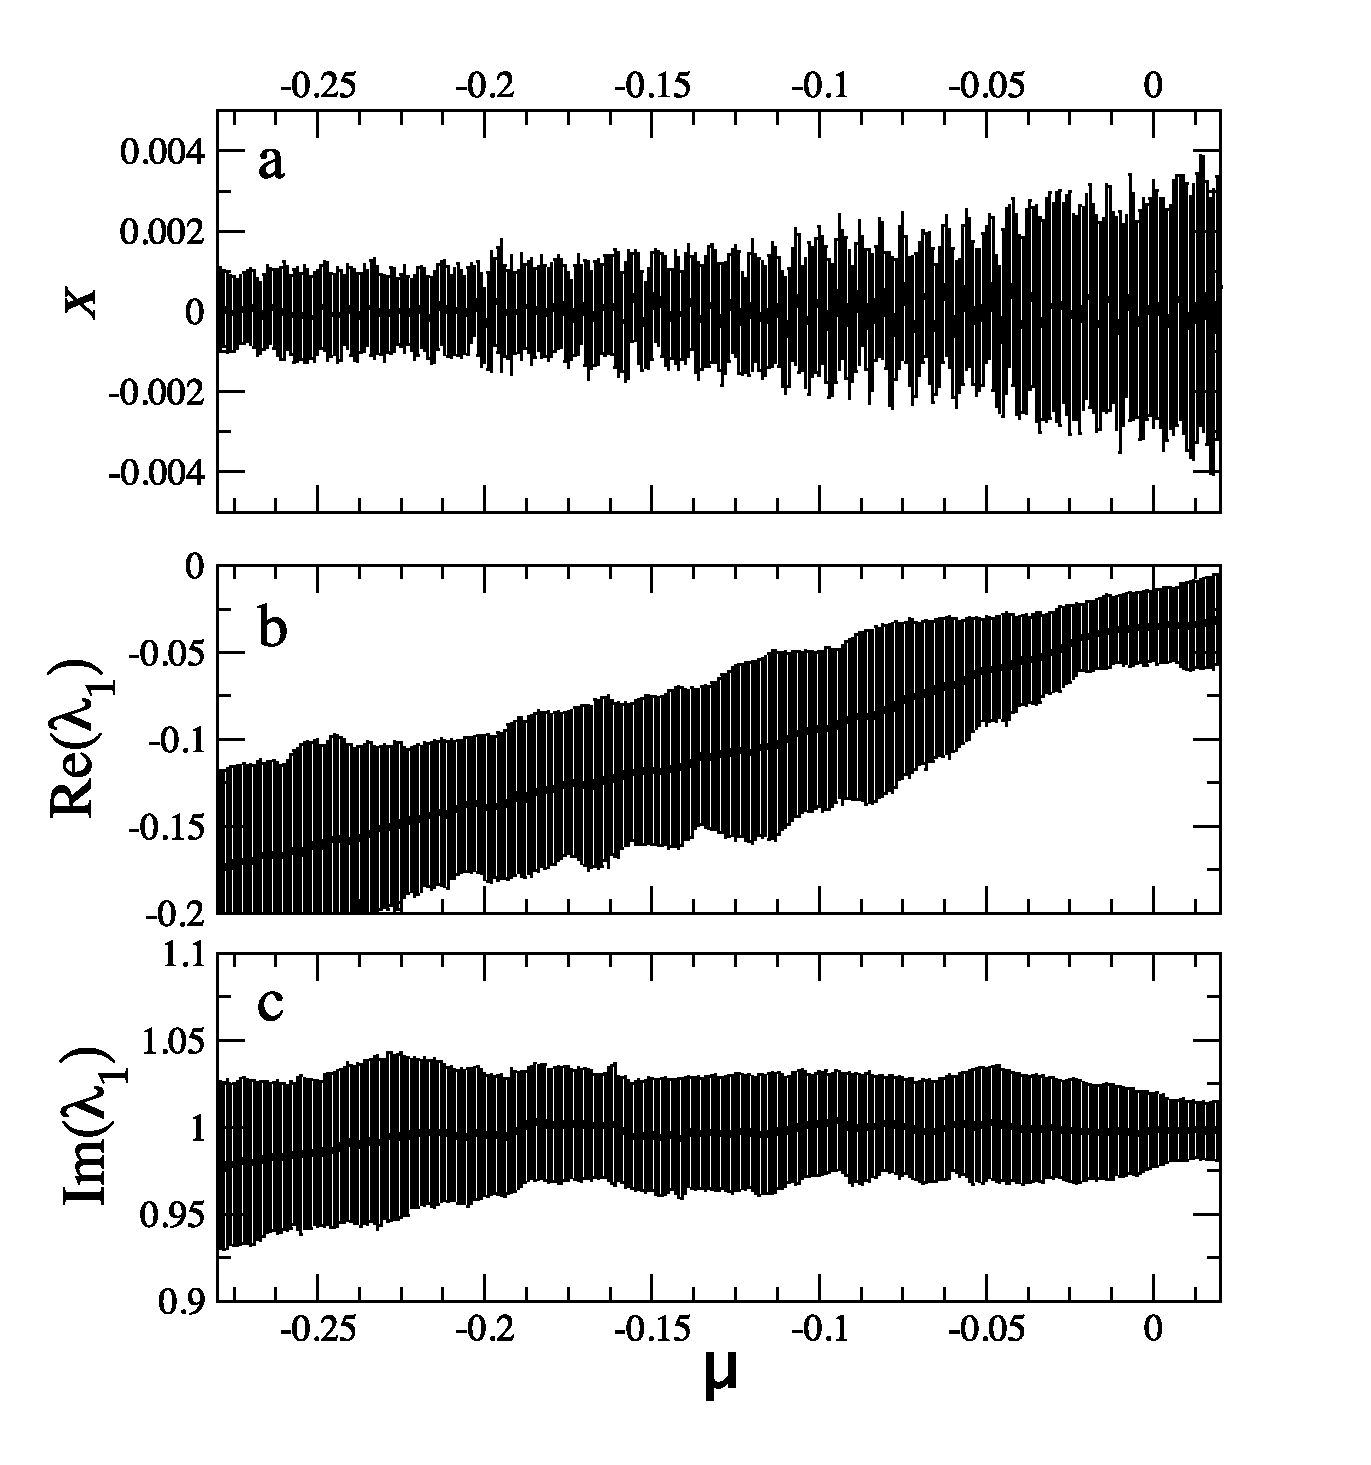
\includegraphics[width = \columnwidth]{02_VDP40}\caption{\label{fig_VDPnoise10} The Van der Pol system described in (\ref{eqn_VDPwithnoise}). (a) The mean of 40 separate trials is shown with error bars of one standard deviation. (b,c) The mean of the first Jacobian eigenvalues are also shown plotted against $\mu$, with error bars of one standard deviation. A Hopf bifurcation occurs at $\mu=0$.}
\end{figure}

In Ref.~\onlinecite{williamson2015}, a method is {\newNote introduced} to anticipate bifurcations in dynamical systems with more than one variable. The method is intentioned as a higher-dimensional analogue of the one-dimensional ACF1 indicator. Indeed, we note the similarities between the equation used to calculate the lag-1 autocorrelation coefficient $a$:
\begin{equation}
a = \frac{ \sum_t (x_{t+1}x_t) - \overline{x}^2}{\sum_t (x_t^2) - \overline{x}^2}\,,
\end{equation} 
and the equation used in Ref.~\onlinecite{williamson2015}:
\begin{equation}
A = \frac{ \sum_t (\x_{t+1}\x_t^\top) - \overline{\x}^2}{\sum_t (\x_t\x_t^\top) - \overline{\x}^2}\, .
\label{eqn_matrixAWilliamson}
\end{equation} 

To illustrate the application of the method, we consider the following example. The system described by (\ref{eqn_hopf}) experiences a Hopf bifurcation at $\mu=0$ if $\mu$ is made to vary with time to approach zero from below. 
\begin{equation}
\begin{array}{rcl}
\dot{r} &=& \mu r - r^3,\\
\dot{\theta} &=& 1 + r^2.
\end{array}
\label{eqn_hopf}
\end{equation} 
The system has stable solution at $r=0$ for $\mu<0$, which becomes unstable when $\mu\geq 0$. We may investigate the nature of the bifurcation by studying the eigenvalues of the Jacobian of the system equations. In Cartesian rather than polar coordinates we have
\begin{equation}
J(x,y) = 
\left(
\begin{array}{cc}
\mu - (x+y)^2-2x^2 & -1-(x+y)^2-2y^2\\
1+(x-y)^2 + 2x^2 & \mu - (x-y)^2-2y^2
\end{array} \right).
\label{eqn_Jacobian_homclinic}
\end{equation} 
At the stable point $r=0$ (i.e. $(x,y)=(0,0)$) this has complex conjugate eigenvalues $\lambda = \mu\pm i$. The system therefore experiences a Hopf bifurcation as $\mu$ approaches zero from below, characterised by the Jacobian eigenvalues moving from the negative-real to the positive-real half of the complex plane.

In Ref.~\onlinecite{williamson2015} a method is described to approximate these Jacobian eigenvalues from the time series in $x$ and $y$. {\noteRed The matrix $A$ (Eqn.~\ref{eqn_matrixAWilliamson}) is used to linearise the system as 
\begin{equation}
\mathbf{x}_t = A\mathbf{x}_{t-1} + \mathbf{c} + \mathbf{\varepsilon}_t,
\label{eqn_AR1analogue}
\end{equation}
where $\mathbf{c}$ is a constant vector and $\mathbf{\varepsilon}_t$ is a white noise term, in which $A = \mathbf{I}+J(\mathbf{x}_\star)\Delta t$. The first order approximation 
\begin{equation}
A = \mathbf{I}+J(\mathbf{x}_\star)\Delta t \approx \exp(J(\mathbf{x}_\star)\Delta t)
\label{eqn_jacobian_justification}
\end{equation}
is used to recover the Jacobian eigenvalues $\lambda_k$ from the eigenvalues $a_k = |a_k|\exp(i\varphi)$ of $A$, with the relations 
\begin{align}
	\begin{split}
		\mathbb{R}(\lambda_k) &= \frac{1}{\Delta t}\ln|a_k| \, ,\\
		\mathbb{I}(\lambda_k) &= \frac{1}{\Delta t} \varphi_k \, .
	\end{split}
	\label{eqn:2D:williamson-eigenvalueRelations}
\end{align}
The eigenvalues $\lambda_k$ are then, themselves,  tipping point indicators.}

By doing this in a sliding window of appropriate length one may note the change in the real part of the eigenvalues and anticipate the bifurcation. Here, we consider another example of a Hopf bifurcation, allowing us to apply this method in a novel system, the Van der Pol oscillator 
\begin{equation}
\ddot{x} - \mu(x-x^2)\dot{x} + x = \eta,
\label{eqn_VDPwithnoise}
\end{equation} 
where the stochastic forcing term $\eta$ is white noise with standard deviation 0.01. We may also write (\ref{eqn_VDPwithnoise}) as a coupled system of first order ODEs:
\begin{equation}
\begin{array}{rcl}
\dot{x} &=& \mu\left(x - \frac{1}{3}x^3\right)+y\,,\\
\dot{y} &=& -x + \eta\,.
\end{array}
\label{eqn_VDPwithnoise_coupled}
\end{equation} 
The {\noteRed zero-noise} system has a stable equilibrium point ($\dot{x}= \dot{y}= 0$) at $(x,y)= (0,0)$ for $\mu<0$ which becomes the centre of a stable limit cycle for $\mu>0$. The Jacobian of this system is given in (\ref{eqn_Jacobian_VDP}). Evaluating the Jacobian matrix $J$ at the stable point $(0,0)$, we find two complex-conjugate eigenvalues $\lambda = \frac{1}{2}(\mu \pm \sqrt{\mu^2-4})$. We therefore expect that the real part of both of the eigenvalues, equal to $\mu/2$, will approach zero as $\mu\rightarrow 0$, i.e. as the system approaches the bifurcation,
\begin{equation}
J(x,y) = \left(
\begin{array}{cc}
\mu(1-x^2) & 1\\
-1 & 0
\end{array}
\right).
\label{eqn_Jacobian_VDP}
\end{equation} 


We integrate the system in (\ref{eqn_VDPwithnoise_coupled}) using a time dependent $\mu(t) = -0.35 + 0.001t$, from $t=0$ to $t=400$. Using the method in Ref.~\onlinecite{williamson2015}, we estimate the first eigenvalue of the Jacobian in a sliding window of 100 points. The mean (with error bars of one standard deviation) of 40 such experiments is show in Fig.~\ref{fig_VDPnoise10}. We note that the real part of the eigenvalue increases as expected and provides an early warning signal of the impending Hopf bifurcation.


\section{Comparison of methods applied to tropical cyclone data}
\label{sec:AppliedHurricanes}
We now apply the methods reviewed in the previous sections to observed geophysical data, {\newNote namely the sea-level pressure (SLP) and wind speed (WS) data from weather stations at the landfall locations of fourteen tropical cyclones, as previously used in Ref.~\onlinecite{prettyman2018}. The physical dynamical system of the atmospheric conditions during the approach of a tropical cyclone exhibits a tipping point, \emph{an abrupt qualitative change in the dynamical system}\cite{scheffer2009,kuehn2011mathematical}, as the cyclone passes by and the SLP dramatically decreases. This tipping has not been modelled as a bifurcation in a dynamical system as has species extinction\cite{drake2010early} and is potentially not a bifurcational or noise-induced tipping point\cite{livina2007,ashwin2012} which are often commonly the targets of early warning signals research\cite{dakos2008,scheffer2009}. However, the principles of tipping point analysis, such as critical slowing down, are sufficiently general\cite{scheffer2009,kuehn2011mathematical} that techniques based on these principles have been applied to a wide variety of physical systems\cite{van2007,dakos2008} without prior knowledge of the tipping present in the system as bifurcational, noise-induced or merely transitional\cite{livina2011,ashwin2012}. The example of the approaching tropical cyclone is used here as a test of tipping point techniques in a novel physical system, the choice of which is supported by the observation that the abrupt decrease in SLP (see Fig.~\ref{fig_ACF1andPS}) constitutes a tipping point in the general sense\cite{scheffer2009critical,kuehn2011mathematical}, and previous results\cite{prettyman2018} showing moderate success with the use of the PS indicator applied to the one-dimensional SLP time series. By inspection, the tipping appears to be transitional\cite{livina2011} rather than bifurcational because of the smooth approach of the cyclone which causes a steady decrease in SLP over a (relatively short) period of a few hours.
}

For each tropical cyclone, we apply EOF to the two times series (SLP and WS) in order to reduce the dimension to one. The time series in both variables are first mean-centred, as per the EOF method, and also normalised in order to non-dimensionalise. {\noteRed A preliminary sensitivity analysis was performed in order to ascertain a general optimal weighting scheme for the variables in the EOF procedure but, with these data, it was not possible to determine an optimal scheme. The two variables are therefore weighted equally, after normalisation.} We are then able to apply the one-dimensional EWS techniques, the ACF1 and PS indicators \cite{prettyman2018} (see Fig.~\ref{fig_ACF1andPS}), and then take the mean over all cyclones. The result is shown in Fig.~\ref{fig_03EOF}: we notice that the rise in the ACF1 indicator (top panel, Fig.~\ref{fig_03EOF}) is more noticeable than when using only the SLP (middle-left panel, Fig.~\ref{fig_ACF1andPS}), but is not so noticeable as when using only the wind speed (middle-right panel, Fig.~\ref{fig_ACF1andPS}). The combination of the two variables using EOF has given an indicator series which appears to be somewhere between the two separate indicator series, although it is not equivalent to simply taking the mean of the two and does give more weight to the more visible indicator. The PS indicator series (bottom panel, Fig.~\ref{fig_03EOF}) is more similar to the PS indicator series using only SLP (bottom-left panel, Fig.~\ref{fig_ACF1andPS}). We quantify the gradient of the indicator by evaluating the Mann-Kendall coefficient of the mean indicator series in the 30-hour window before time zero, using the equation
\begin{equation}
\sum_{i=1}^{N-1}\sum_{j=i+1}^{N}\text{sign}(X_j-X_i)\,,
\label{eqn_MK}
\end{equation} 
where $X$ is the time series of the indicator. The result is summarised in table~\ref{tab_EOFresults}.

\begin{table}
\centering
\begin{tabular}{ccc}
\hline
& \multicolumn{2}{c}{Indicator} \\
\cline{2-3}
Data & ACF1 & PS\\
\hline
Sea-level pressure & -0.2 & 0.79 \\
Wind speed & 0.91 & 0.70 \\
EOF & 0.45 & 0.72\\
\hline
\end{tabular}

\caption{Comparison of the gradient of the indicator of the time series data in a 30-hour window before the tropical cyclone event. We compare sea-level pressure and wind speed data alone (as presented in Fig.~\ref{fig_ACF1andPS}) to the first EOF score of the two series (Fig.~\ref{fig_03EOF}). In the case of each indicator (ACF1 and PS), the indicator applied to the first EOF score has a gradient somewhere between the two considered alone.}\label{tab_EOFresults}
\end{table}

The method of approximating Jacobian eigenvalues has previously been applied to dynamical systems where the governing equations and the type of bifurcation are known \cite{williamson2015}, and so we know in advance what type of signal we should expect, such as with our Van der Pol example (Fig.~\ref{fig_VDPnoise10}). However, we have noted that the method was intentioned as a two-dimensional analogue to the lag-1 autocorrelation {\newNote which is applicable in wide variety of dynamical systems exhibiting tipping points\cite{van2007,dakos2008,livina2011,ashwin2012} due to the generality of the the critical slowing down phenomenon\cite{scheffer2009,kuehn2011mathematical}. It is reasonable, therefore, to test this technique} on our SLP/WS system in which the ACF1 indicator increases prior to the tropical cyclone event. Fig.~\ref{fig_03WL} shows the result of applying this method to the SLP and WS variables simultaneously. As with the EOF method, the time series in both variables are mean-centered and normalised in the implementation of this method. The real parts of the first and second Jacobian eigenvalues are shown (top and bottom panels respectively). We note that the real part of the first eigenvalue increases prior to the event, similar to the ACF1 and PS indicators in Fig.~\ref{fig_03EOF}.

\begin{figure}
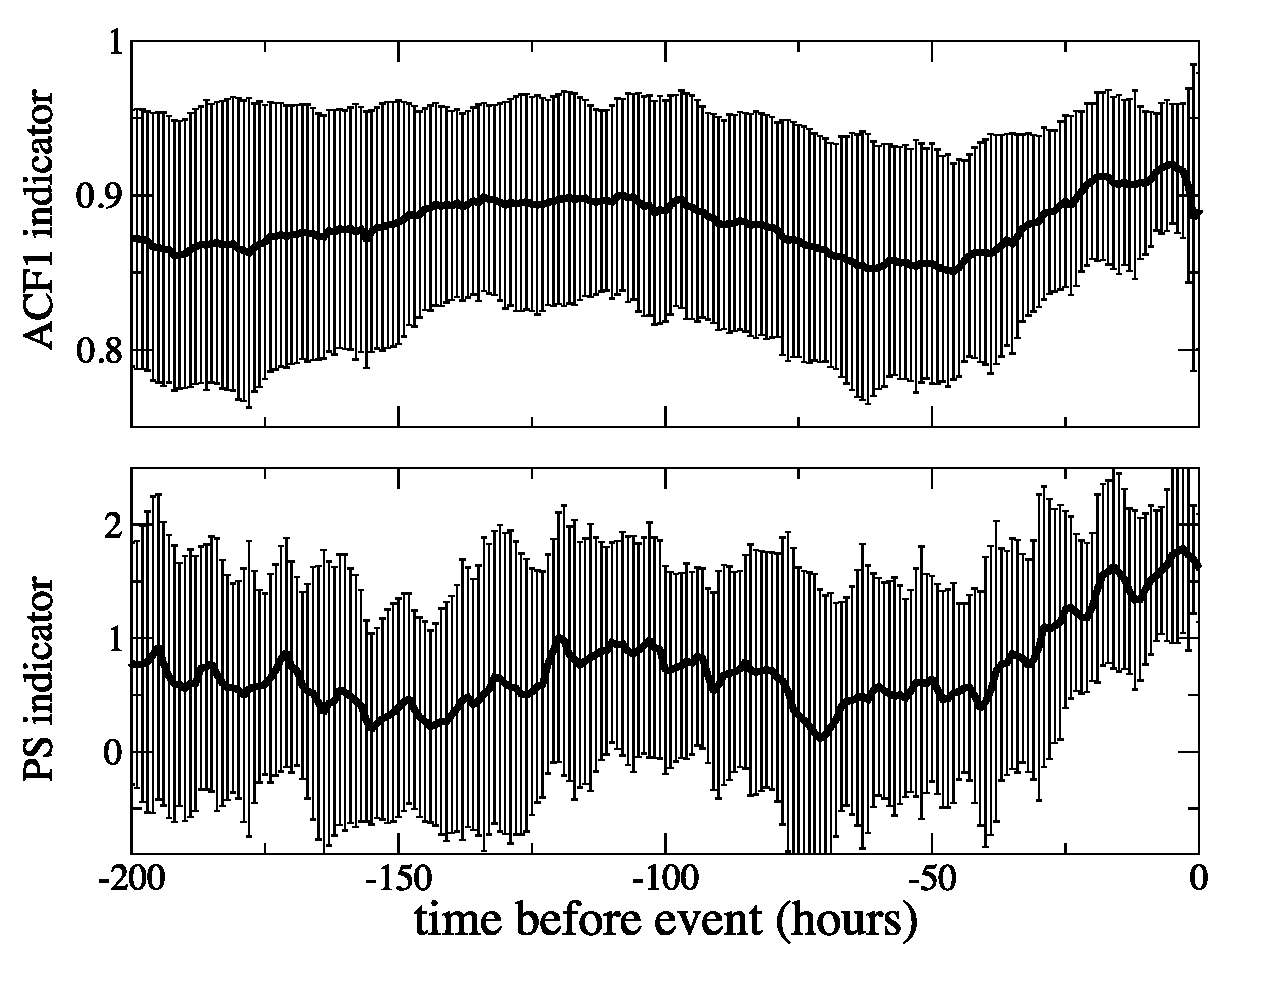
\includegraphics[width = \columnwidth]{03_EOF}\caption{\label{fig_03EOF} EWS analysis of the first EOF score of tropical cyclone data using scaling indicators. The mean ACF1 indicator (top) and PS indicator (bottom) of the first EOF scores calculated from the wind speed and sea-level pressure.}
\end{figure}
\begin{figure}
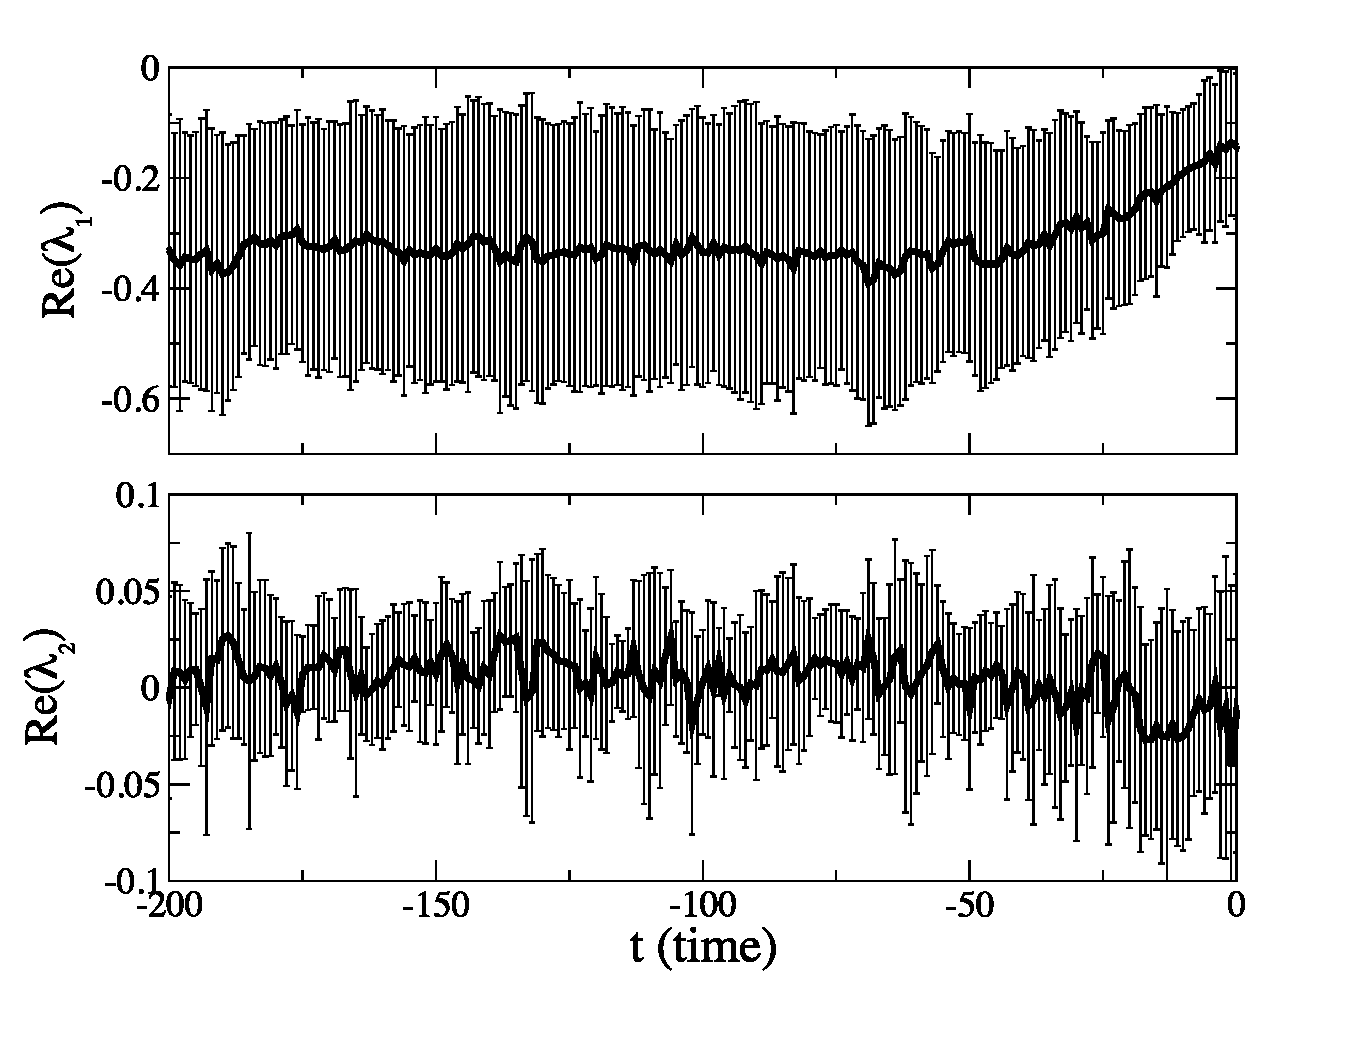
\includegraphics[width = \columnwidth]{04_WL}\caption{\label{fig_03WL} EWS analysis of tropical cyclone data using the method described in Ref.~\onlinecite{williamson2015}. The real part of the first and second Jacobian eigenvalues ($\lambda_1$ and $\lambda_2$). We note that the real part of the first eigenvalue appears to increase, although not significantly, prior to the event.}
\end{figure}
%\begin{figure}
%\includegraphics[width = \columnwidth]{../figures/03_EOFvsWL}\caption{\label{fig_EOFvsWL} (a) The mean ACF1 indicator of the first EOF scores calculated from the wind speed and sea-level pressure. (b,c) The real part of the first and second Jacobian eigenvalues ($\lambda_1$ and $\lambda_2$). We note that the real part of the first eigenvalue appears to increase, although not significantly, prior to the event.}
%\end{figure}

\section{Analysis of multiple time series}
\label{sec:MultipleTimeSeries}
Here we make an attempt to use the one-dimensional EWS indicators\cite{prettyman2018} applied to multiple time series data distributed over a geographic area. By using more data we expect to improve the performance of the EWS techniques. We also investigate the spatial variation in the indicator series, potentially with a view towards detecting a spatial pattern which may provide a warning of the arrival of the tropical cyclone.
We investigate eight different cyclones which have made landfall on the Caribbean or Florida coastlines of the United States, these are given in table \ref{tab_hurricanes}. Hurricane Andrew appears twice (labeled Andrew 1 and Andrew 2) because it made landfall twice: over Florida and then, two days later, over Louisiana. We therefore have a total of nine hurricanes. Again, we use the HadISD 2017 data set \cite{HadISD,HadISD_dunn12,HadISD_dunn14,HadISD_dunn16,HadISD_smith} and take data from stations within 200km of the landfall. Only hurricanes making landfall over the United States mainland were selected because there is usually a relatively high density of data points supplied by the dataset, in comparison to Mexico and other Caribbean nations. 


\begin{table}
	\centering
	\begin{tabular}{ l  l  l  c }
		\hline
		Name & Date & Region & Entry point\\
		\hline \hline
		Andrew 1 &  24 August 1992 &      Florida     &   [25.4N,    -79.0E]\\
		
		Andrew 2 &  26 August 1992 &      Louisiana  &  [29.8N,  -91.6E]\\
		
		Katrina &   29 August 2005 &     Louisiana &   [29.3N,   -89.6E]\\
		
		Wilma &     24 October 2005 &   Florida     &   [25.3N,    -82.7E]\\
		
		Gustav &  1 September 2008 &   Louisiana & [29.3N,    -90.8E]\\
		
		Matthew &  7 October 2016 & Florida     & [26.7N,    -79.0E]\\
		
		Harvey  &  25 August 2017 &      Texas       &  [25.2N,    -94.6E]\\
		
		Irma &        10 September 2017 & Florida    &  [24.5N,    -81.5E]\\
		
		Nate &       8 October 2017 &    Louisiana &   [29.3N,   -89.2E]\\
		\hline
	\end{tabular}
\caption{The dates and locations of each of the nine hurricanes considered. The entry point coordinates column gives the points at which each hurricane entered the region we are considering in each case (defined by a minimal rectangle containing all of the weather stations used). Hurricane Andrew appears twice (labeled Andrew 1 and Andrew 2) because it made landfall twice: over Florida and then, two days later, over Louisiana.}\label{tab_hurricanes}
\end{table}

For each of the nine hurricanes, we take the SLP variable data from all available stations in the region supplied by the HadISD 2017 dataset. We then calculate the PS indicator series for each pressure series and asses the slope of that indicator series, using the Mann-Kendall coefficient, in a window of approximately 30 hours before the hurricane enters the region. If the behaviour here is similar to the behaviour of the mean of the PS indicator applied to the individual sea level pressure series (Fig.~\ref{fig_ACF1andPS} bottom left) we would expect that an upward trend in the indicator (i.e. a high value of the Mann-Kendall coefficient) will be detectable for each location within 30-hours travelling time of the hurricane. We expect that the slope of the PS indicator series would be high at points where the hurricane is very close and lower at points further from the point where the hurricane enters the region. 

The slope of the PS indicator is assessed, in each case, using the Mann-Kendall coefficient given by (\ref{eqn_MK}). The window size used in the calculation of the PS indicator series, and the length of the window in which the Mann-Kedall coefficient is evaluated, are determined for each hurricane through a sensitivity analysis (see supplementary material). Here, the increase in the indicator is usually seen in a 30-50 hour window before the event, which is consistent with our expectations. We therefore measure the Mann-Kendall coefficient of the indicator series (for the time series at each spatial location, separately) in a 30-50 hour window before a time $T_{\text{entry}}$ which is the time at which the cyclone enters the region under study, that is the time at which the minimum pressure is attained at the first spatial location on the cyclone's path. We expect to see a high coefficient value (i.e. a large increase in the indicator) at locations close to the entry point.

Also, according to the sensitivity analysis, we note that the PS indicator is most useful when using a window size which is an odd multiple of six, consistent with the result of the similar sensitivity analysis in Ref.~\onlinecite{prettyman2018}. This is likely due to tidal oscillations in the data. We have chosen an indicator window size of either 90 or 102 points depending on the hurricane.

The value of the Mann-Kendall coefficient of the PS indicator is plotted as a filled contour plot over the geographic area. In Fig.~\ref{fig_ContourMapSummary} we present a summary of the results: in each case, the contour map is rotated so that the forward path of the Hurricane is moving from the bottom to the top of the image. Hurricane tracks, obtained from the NOAA HURDAT2 dataset \cite{HURDAT2}, are shown by the black line. We are generally able to see a movement of the hurricane from areas with a high value of the Mann-Kendall coefficient, towards areas with lower value, as we expect. Whilst this doesn't provide a useful EWS, it is clear that the PS indicator is more robust when applied to many time series in a region than when applied to individual series, as in Fig.~\ref{fig_ACF1andPS}.

\begin{figure}
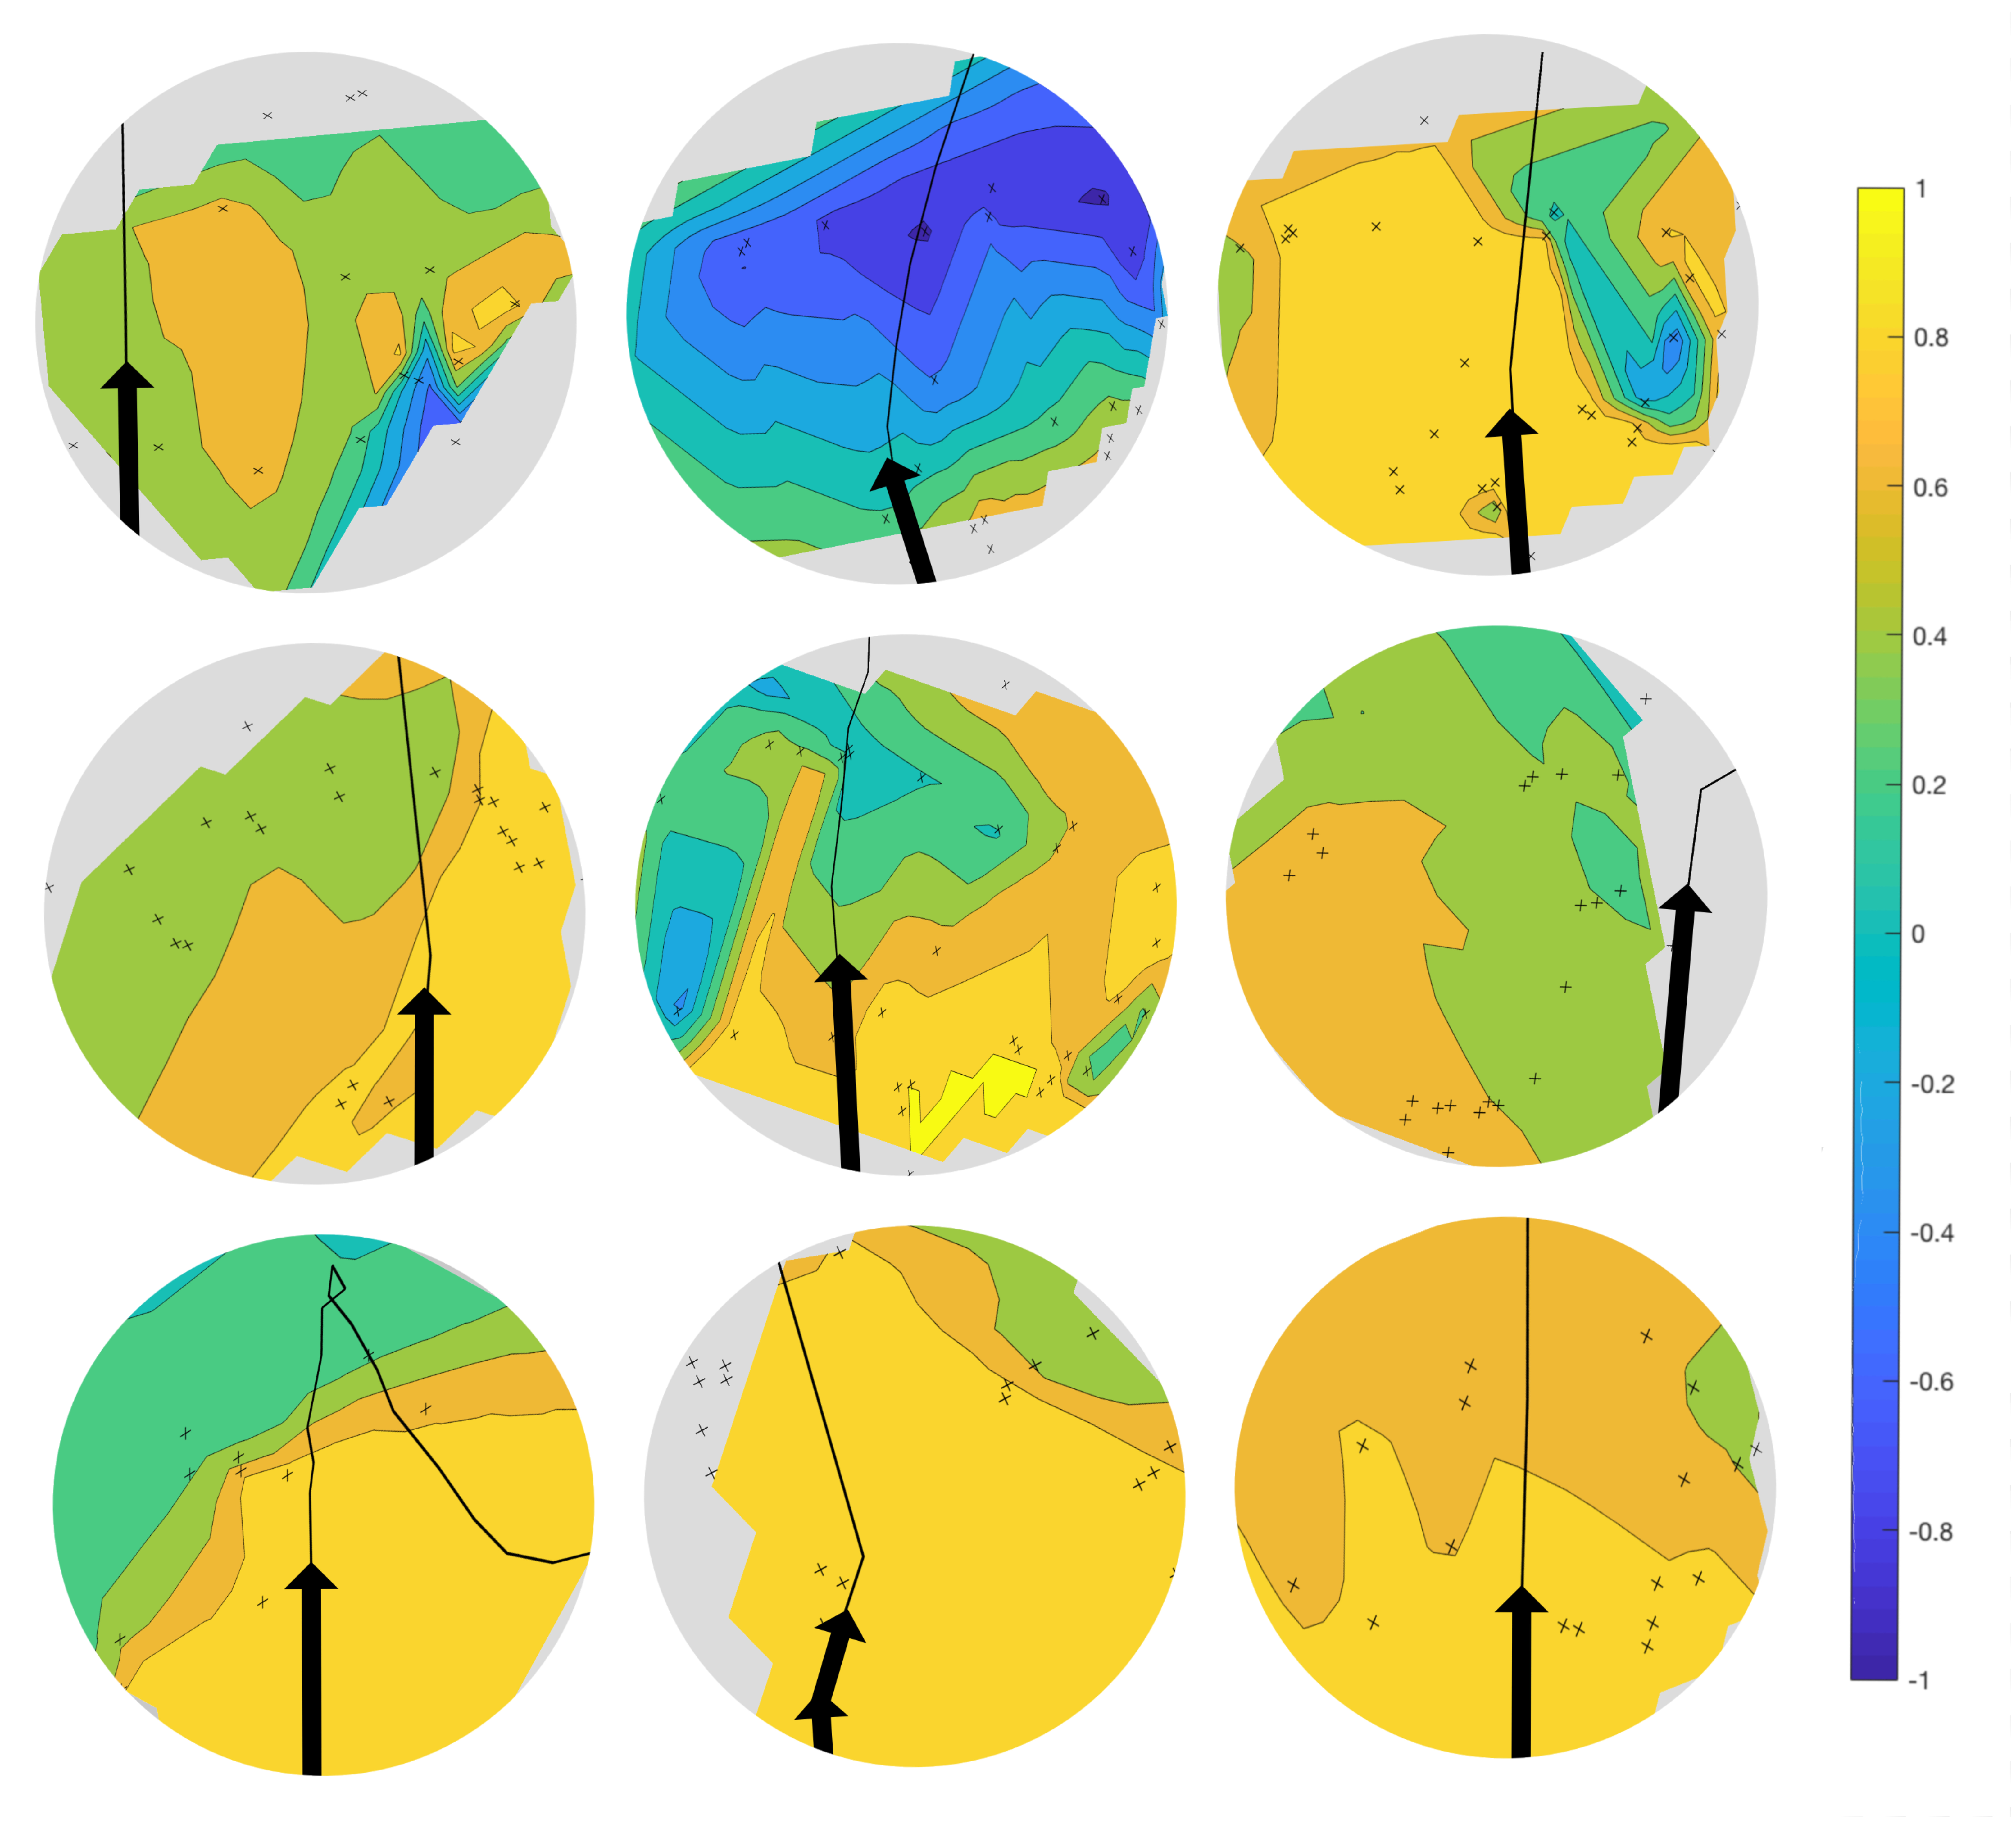
\includegraphics[width = \columnwidth]{05_Contour3x3}
\caption{Contour plots of PS indicator gradient for nine Atlantic hurricanes on the Caribbean and Florida coastlines of the USA. left to right: Andrew (Florida); Andrew (Louisiana); Katrina; Wilma; Gustav; Matthew; Harvey; Irma; Nate. In each case, the slope of the PS indicator is evaluated using the Mann-Kendall coefficient and the value of this coefficient is plotted over the geographic area. Each plot has been rotated so that the hurricane track is moving from the bottom to the top of the image (shown by the black line, direction indicated by thick black arrow). The locations of the weather stations are shown by crosses; the grey areas fall outside of the polygon enclosing the weather stations and are therefore not interpolated onto.}
\label{fig_ContourMapSummary} 
\end{figure}

\section{A simple model of the approaching cyclone}
\label{sec:Model}

Ref.~\onlinecite{holland1980} presents a simple analytic model of the pressure ($p$) profile in hurricanes:
\begin{equation}
p(r) = p_c + (p_n-p_c)\exp\left( \frac{-A}{r^B} \right),
\label{eqn_hollandmodel}
\end{equation} 
where $r$ is the radial distance from the centre of the hurricane, $p_c$ and $p_n$ are the central and ambient pressures, $A$ and $B$ are parameters to be determined by fitting to observed data. Ref.~\onlinecite{holland1980} fits the model to three Australian hurricanes: Tracy (December 1974), Joan (December 1975) and Kerry (February 1979). The values of parameters $A$ and $B$ are obtained by fitting to sparse observations, particularly observations of maximum wind speed $V_m$ given by
\begin{equation}
V_m = \left(\frac{B(p_n-p_c)}{\rho e}\right)^{1/2},
\end{equation} 
and occurring at a radius $R_w = A^{1/B}$. 

Here we present a similar model modified so that the pressure is modelled at a fixed point in space as a function of time, rather than a profile modelled at a fixed time as a function of the distance from the hurricane centre. We are therefore able to model the effect on sea level pressure (at a weather station, for example) of an approaching hurricane. 
We use the values $A=40$ and $B=1$ which are obtained by fitting to Hurricane Katrina (2005) at peak intensity. We consider a fixed point at distance~$d(t)$ from the hurricane centre at time~$t$. In (\ref{eqn_hollandmodel}) we replace $r$ by $d(t)$ to introduce a time dependence. We assume the hurricane moves in a straight line towards the fixed point with a speed of $v(t)$kmh$^{-1}$, in which case we have $d(t) = \int_0^t v(s) ds$. For this model, a constant volocity will suffice: 18kmh$^{-1}$ is obtained by taking a mean of the tropical cyclones studied in Ref.~\onlinecite{prettyman2018}, we therefore use a velocity chosen uniformly from the range~$[16,20]$ so that not all implementations of the model are identical. The ambient pressure, $p_n$, is given by 
\begin{equation}
p_n(t) = 1016 + 5\eta_1 + 1.6\sin\left(\frac{2\pi t}{12} + K\right),
\label{eqn_ambientpressure}
\end{equation} 
where $K$ is a random offset chosen uniformly in the range $[0,12]$, the sine wave models the 12-hourly tidal oscillations. The central pressure is given by $p_c = 950+10\eta_2$. Values $\eta_1$ and $\eta_2$ are sampled from a standard normal distribution. The reason for the inclusion of $\eta_1$, $\eta_2$ and the random offset $K$ is that we may wish to run the model multiple times and take the mean of statistics over those simulations to obtain an ensemble estimate. For this purpose, we would not want all of the sine wave components to be aligned, nor for all the models to have exactly the same initial parameters.

There is also a need to model the increasing PS indicator value shown to exist in the pressure signal. We therefore add a noise signal to the output in which the power spectrum scaling exponent, $\alpha$, increases over time. The maximum value of $\alpha$ is greater for points closer to the cyclone track, and the time at which the maximum value is reached is the time at which the closest approach occurs, which we call $T_{\min}$. We have used values  {\newNote such that $\alpha$ for $t<T_{\min}-50$ (more than fifty hours before the minimum approach distance is reached). In the 50-hour window before the minimum approach distance, the value of $\alpha$ increase linearly from the background value of $0.4$ to a higher value $\alpha_0$ which takes the value 2 in cases where the hurricane path passes directly over the grid-point in question (an approach distance of zero) and decreases linearly with increasing distance from the cyclone track, to a minimum value of $0.4$ for grid-points more than 200km distant.}

The part of the noise signal with increasing $\alpha$ value is made by concatenating 10 sub-series, each of length 1000 and with a higher $\alpha$ value than the last (covering the range $[0.4, \alpha_0]$), then sampling with an interval size chosen to give a series of the desired length. All of the noise signals in the model are generated by the coloured noise generation method detailed in Ref.~\onlinecite{kasdin1995}. 

 This artificial noise is then added to the model simply to reproduce the increase in PS indicator without introducing a large increase in the ACF1 indicator. That is, we have parametrised the stochastic component of the model using the behaviours of the indicators applied to the data presented in Fig.~\ref{fig_ACF1andPS}.

We therefore have the model:
\begin{equation}
p(d(t)) = p_c + (p_n(t)-p_c)\exp\left( \frac{-A}{d(t)^B} \right) + \eta_t,
\label{eqn_OurOwnModel}
\end{equation} 
where $d(t)$ distance to the centre of the hurricane at time $t$, $p_c$ is the central pressure, $p_n(t)$ is the ambient pressure at time $t$ given by (\ref{eqn_ambientpressure}), $A=40$ and $B=1$ are fitted parameters, and $\eta_t$ is a noise term with changing power spectrum scaling exponent as described above. {\newNote In order to successfully model a tipping point\cite{scheffer2009,kuehn2011mathematical}, the noise term is relatively small compared to the deterministic effect of the exponential term which governs the abrupt transitional tipping\cite{livina2011} from the high-pressure state to the low-pressure state.} For every point on a spatial grid we are able to calculate the distance $d(t)$ using simple geometry (we model the hurricane as moving in a straight line), generate the noise series $\eta$ and then calculate the pressure at that point using (\ref{eqn_OurOwnModel}). 

We model sea-level pressure at a single point in space which is approached by a hurricane passing by at a distance of 20km, the model uses a time-step of 0.05 hours and 100 implementations are evaluated. We then calculate the ACF1- and PS indicators in a 100-hour sliding window in order to compare with the results in Fig.~\ref{fig_ACF1andPS} and in Ref.~\onlinecite{prettyman2018}. The result is shown in Fig.~\ref{fig_model100}. We see that the ACF1- and PS indicators behave similarly to the result from the real sea-level pressure data, and the pressure series itself also looks reasonable. 

\begin{figure}
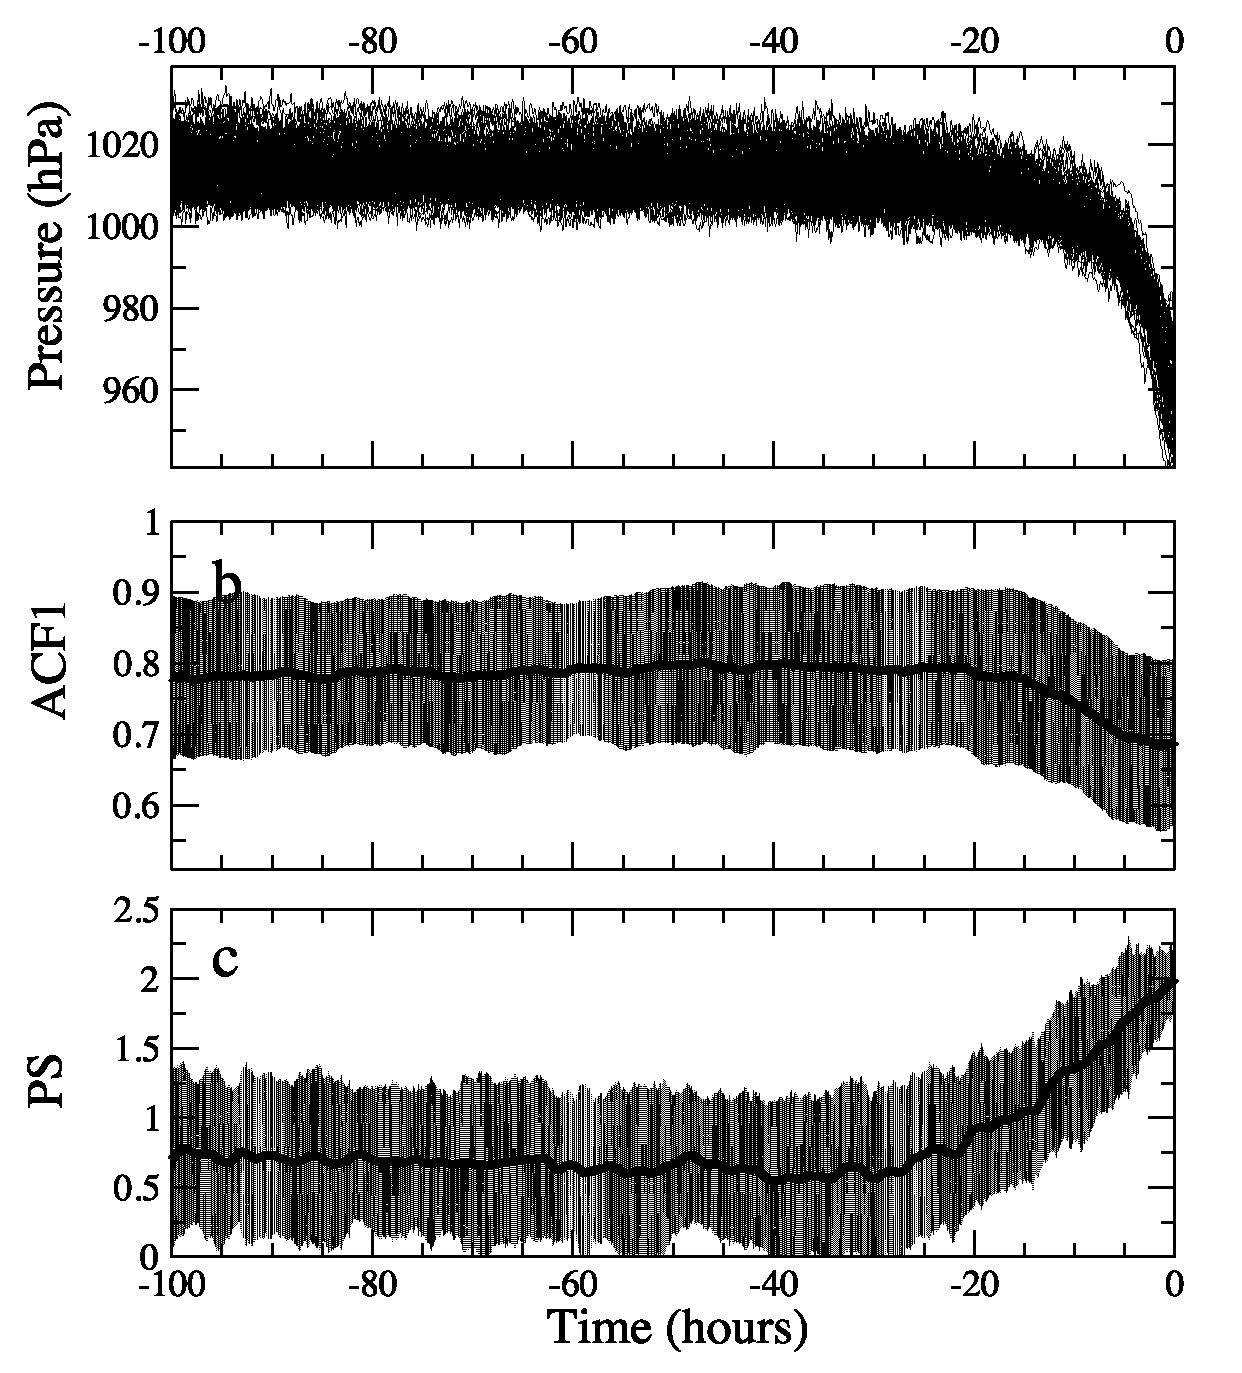
\includegraphics[width = \columnwidth]{06_simpleModel100}\caption{\label{fig_model100} Model data (see (\ref{eqn_OurOwnModel})) and its EWS indicators. (top) 100 runs of the model with (middle) the mean ACF1 indicator and (bottom) the mean PS indicator, shown with error bars of one standard deviation.}
\end{figure}

The model is then evaluated with a time-step of 0.05 hours at 100 points in a ten-by-ten grid with 40km spatial separation between points (giving a square of side 360km). The hurricane is modelled as travelling from 'south' to 'north' from 400 hours before reaching the bottom of the grid up to the point where it reaches the top of grid. The PS indicator of the pressure signal for each grid-point is calculated in a 100-hour sliding window (of 20,000 points). We then calculate the PS indicator slope, evaluated using the Mann-Kendall coefficient in the exact same way as shown in the previous section (Fig.~\ref{fig_ContourMapSummary}), in the 30-hour window before the hurricane reaches the bottom of the grid. Fig.~\ref{fig_tenModelRuns} shows the mean over ten such evaluations for ten separate runs of the model. We see that the pattern is consistent with our expectations and also with the general pattern of the analysis of real data in Fig.~\ref{fig_ContourMapSummary}. 

\begin{figure}
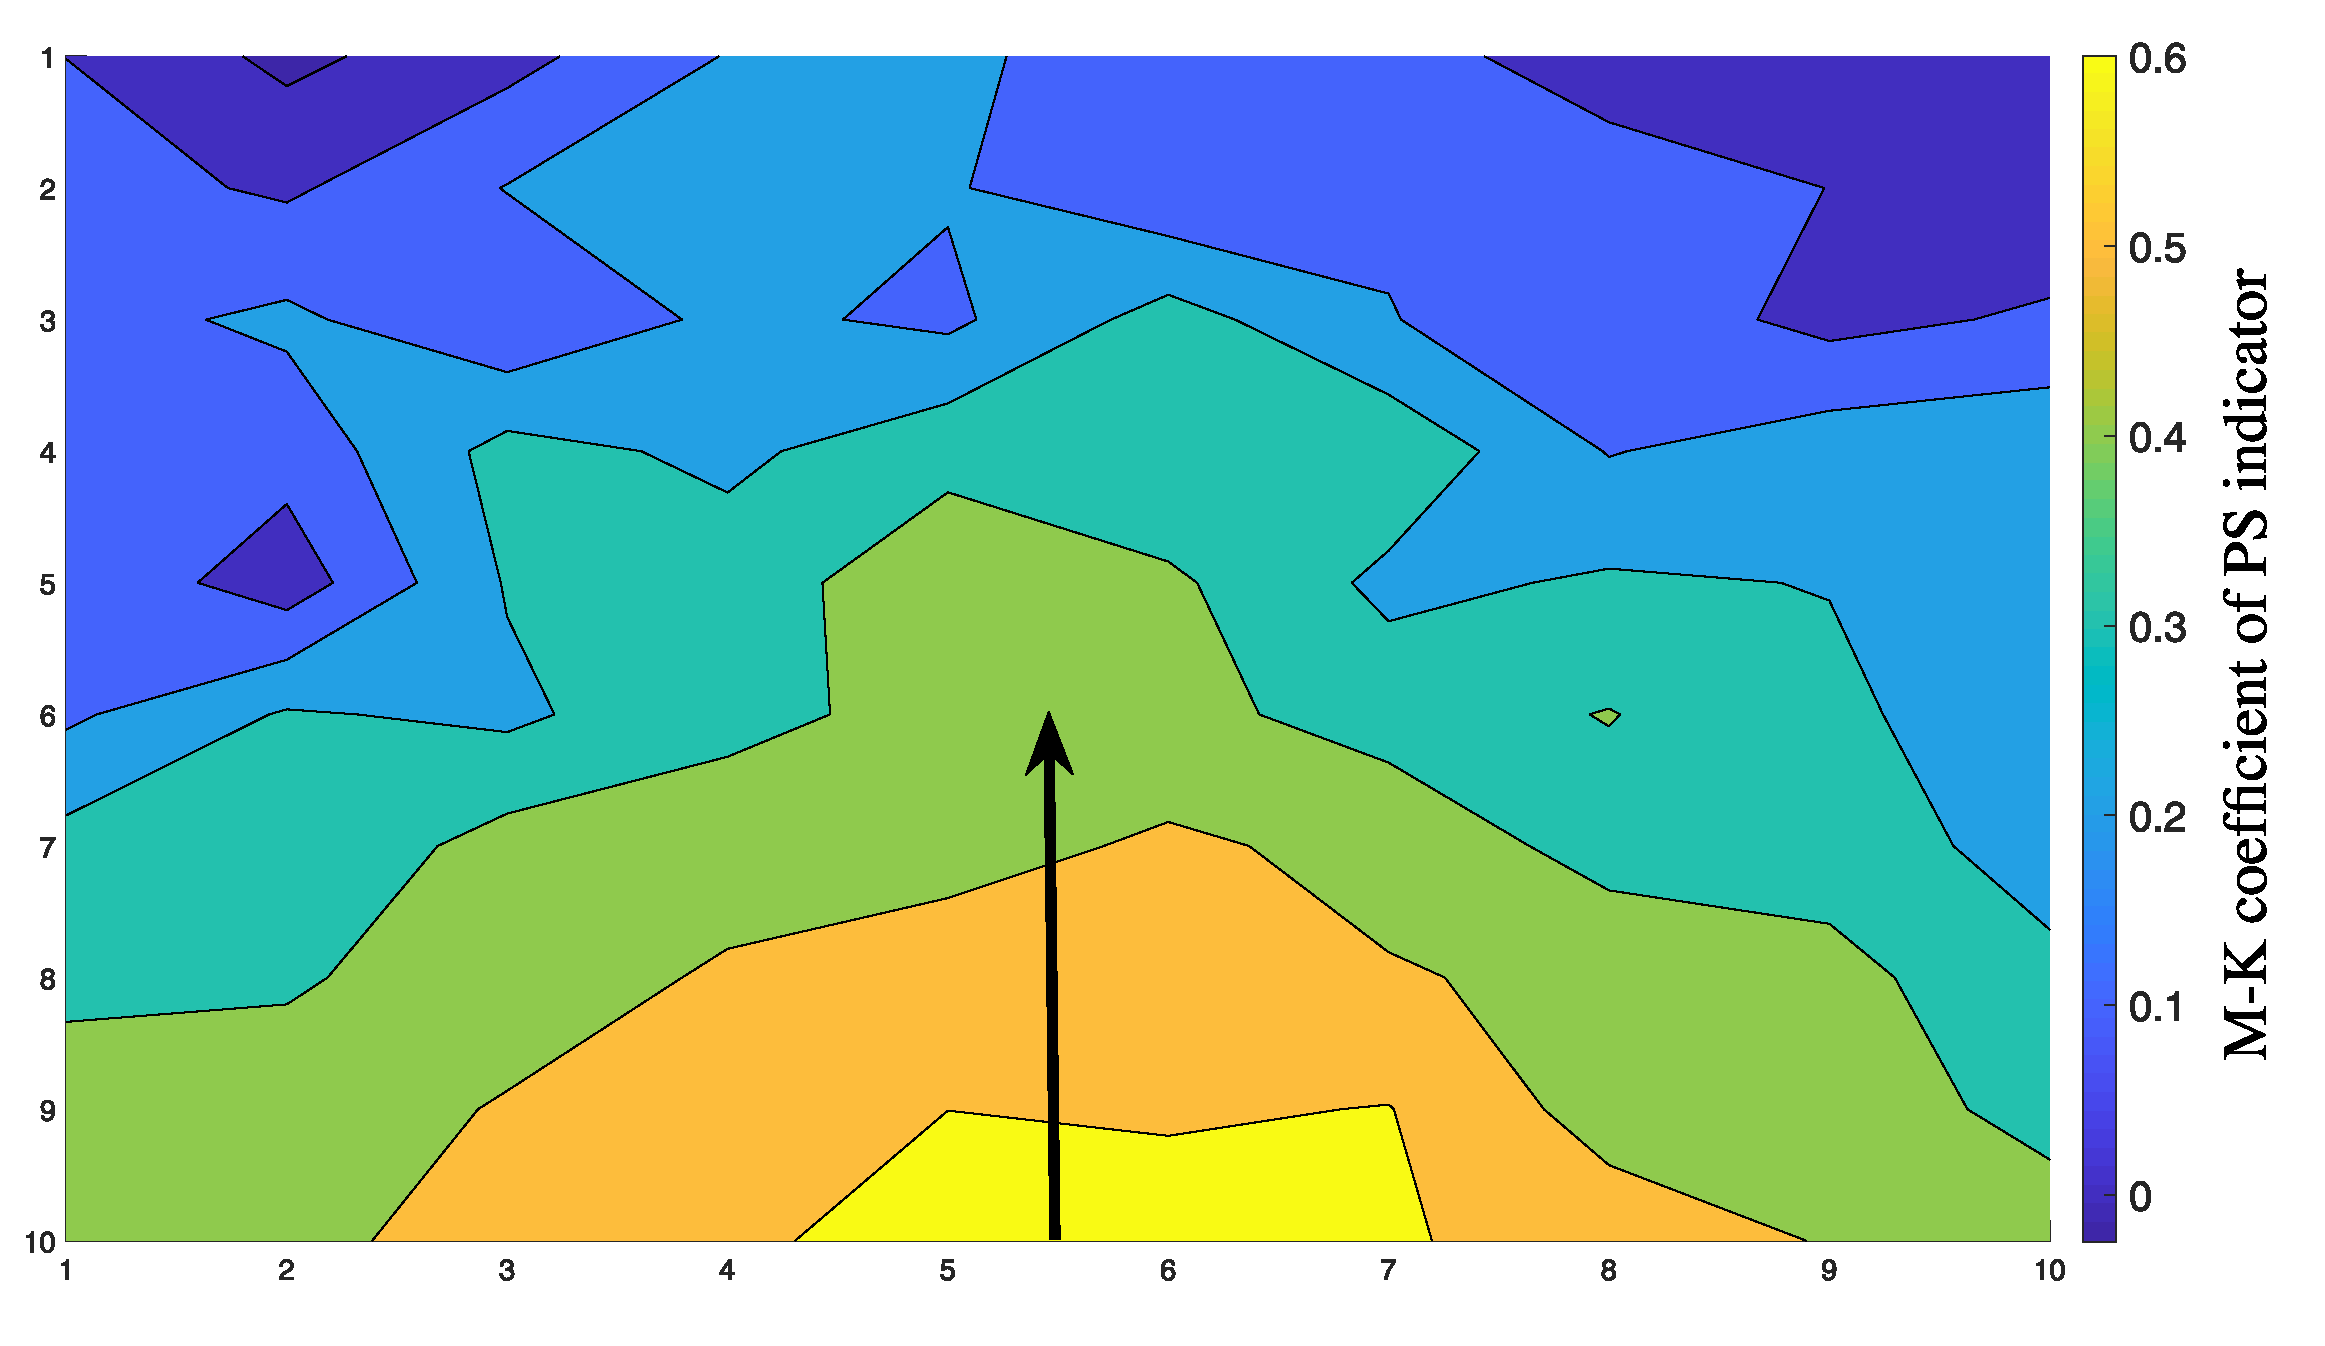
\includegraphics[width = \columnwidth]{07_tenModelRuns}\caption{\label{fig_tenModelRuns} Showing the mean over ten realisations of the model of the PS indicator slope calculated using the Mann-Kendall coefficient. The slope is evaluated for the PS indicator of the pressure signal at each of 100 grid points with 20km spacing, in a 30-hour window before the modelled hurricane reaches the bottom of the image. The forward motion of the hurricane is shown by the black arrow.}
\end{figure}

\section{Summary}
\label{sec:Summary}
The one-dimensional EWS techniques we have used previously \cite{prettyman2018} have been extended to a two-variable system by first using EOF to reduce the dimension. We have shown that in a general {\noteRed linear} dynamical system it is likely to be true that the EOF technique, which projects a system onto a vector which maximises its variance, will also tend to project onto the vector relevant to the tipping point. Because of this, it is likely that typical EWS techniques would be useful in systems where EOF dimension-reduction has been used.
We have demonstrated this with data from points close to tropical cyclones. The ACF1 indicator applied to the sea-level pressure time series does not show any EWS, whereas when applied to the wind speed data an increase can be seen in the mean. When applied to the EOF of both variables, we are also able to detect an increase. The result is also true of the PS indicator. However, EOFs are ``not designed to reveal the structure of the time evolution of the [dynamical] system'' \cite{hasselmann1988} and Principal oscillation patterns (POPs) \cite{von1995} may therefore be better suited to EWS applications. This is an important future step in multi-dimensional EWS detection. We have also applied the method described imn Ref.~\onlinecite{williamson2015} to the same tropical cyclone data and found that there is detectable EWS.

We have also applied the one-dimensional PS indicator to multiple time series distributed spatially. The PS indicator does consistently rise in the 30-hour window before a hurricane. In addition, a model of an approaching hurricane has been presented in order to aid the study of the EWS indicator, and it has been found to agree with the real data, confirming our understanding of the statistics.

We suggest the methods studied in this paper for the tipping-point analysis of multivariate time series data. Multivariate data may be analysed using one-dimensional indicators, the most common of which are the variance and the lag-1 auto-correlation, after reducing the dimension using EOF. It is also possible to use the eigenvalues of the Jacobian matrix of the system as an indicator, which can be estimated from the time series analogously to the one-dimensional indicator methods \cite{williamson2015}. In systems over a two-dimensional field (such as geophysical gridded data), one-dimensional EWS indicators may be evaluated at every point to produce a heat map of the indicator over the area. This may provide a useful EWS; provide an insight into the performance of different indicators; or provide insights into the statistical or dynamical properties of the system (possibly for the purpose of modelling). 

We have applied these methods to tropical cyclones and suggest that they can be applied to a variety of tipping-point phenomena (such as landslides) where high-resolution data is available. 

\section*{Supplementary Material}
\label{sec:Supplementary}

See supplementary material for detail of the sensitivity analysis performed prior to the application if the PS indicator upon sea-level pressure data in Sec.~\ref{sec:MultipleTimeSeries}.

\section*{Acknowledgements}
\label{sec:Acknowledgements}

This paper is the result of a PhD project supported by the EPSRC Mathematics of Planet Earth centre for doctoral training, the National Physical Laboratory and the NERC National Centre for Earth Observation.
	
\bibliography{}

%merlin.mbs aipnum4-1.bst 2010-07-25 4.21a (PWD, AO, DPC) hacked
%Control: key (0)
%Control: author (8) initials jnrlst
%Control: editor formatted (1) identically to author
%Control: production of article title (0) allowed
%Control: page (1) range
%Control: year (1) truncated
%Control: production of eprint (0) enabled
\begin{thebibliography}{34}%
	\makeatletter
	\providecommand \@ifxundefined [1]{%
		\@ifx{#1\undefined}
	}%
	\providecommand \@ifnum [1]{%
		\ifnum #1\expandafter \@firstoftwo
		\else \expandafter \@secondoftwo
		\fi
	}%
	\providecommand \@ifx [1]{%
		\ifx #1\expandafter \@firstoftwo
		\else \expandafter \@secondoftwo
		\fi
	}%
	\providecommand \natexlab [1]{#1}%
	\providecommand \enquote  [1]{``#1''}%
	\providecommand \bibnamefont  [1]{#1}%
	\providecommand \bibfnamefont [1]{#1}%
	\providecommand \citenamefont [1]{#1}%
	\providecommand \href@noop [0]{\@secondoftwo}%
	\providecommand \href [0]{\begingroup \@sanitize@url \@href}%
	\providecommand \@href[1]{\@@startlink{#1}\@@href}%
	\providecommand \@@href[1]{\endgroup#1\@@endlink}%
	\providecommand \@sanitize@url [0]{\catcode `\\12\catcode `\$12\catcode
		`\&12\catcode `\#12\catcode `\^12\catcode `\_12\catcode `\%12\relax}%
	\providecommand \@@startlink[1]{}%
	\providecommand \@@endlink[0]{}%
	\providecommand \url  [0]{\begingroup\@sanitize@url \@url }%
	\providecommand \@url [1]{\endgroup\@href {#1}{\urlprefix }}%
	\providecommand \urlprefix  [0]{URL }%
	\providecommand \Eprint [0]{\href }%
	\providecommand \doibase [0]{http://dx.doi.org/}%
	\providecommand \selectlanguage [0]{\@gobble}%
	\providecommand \bibinfo  [0]{\@secondoftwo}%
	\providecommand \bibfield  [0]{\@secondoftwo}%
	\providecommand \translation [1]{[#1]}%
	\providecommand \BibitemOpen [0]{}%
	\providecommand \bibitemStop [0]{}%
	\providecommand \bibitemNoStop [0]{.\EOS\space}%
	\providecommand \EOS [0]{\spacefactor3000\relax}%
	\providecommand \BibitemShut  [1]{\csname bibitem#1\endcsname}%
	\let\auto@bib@innerbib\@empty
	%</preamble>
	\bibitem [{\citenamefont {Held}\ and\ \citenamefont
		{Kleinen}(2004)}]{held2004}%
	\BibitemOpen
	\bibfield  {author} {\bibinfo {author} {\bibfnamefont {H.}~\bibnamefont
			{Held}}\ and\ \bibinfo {author} {\bibfnamefont {T.}~\bibnamefont {Kleinen}},\
	}\bibfield  {title} {\enquote {\bibinfo {title} {Detection of climate system
				bifurcations by degenerate fingerprinting},}\ }\href@noop {} {\bibfield
		{journal} {\bibinfo  {journal} {Geophysical Research Letters}\ }\textbf
		{\bibinfo {volume} {31}} (\bibinfo {year} {2004})}\BibitemShut {NoStop}%
	\bibitem [{\citenamefont {Dakos}\ \emph {et~al.}(2008)\citenamefont {Dakos},
		\citenamefont {Scheffer}, \citenamefont {van Nes}, \citenamefont {Brovkin},
		\citenamefont {Petoukhov},\ and\ \citenamefont {Held}}]{dakos2008}%
	\BibitemOpen
	\bibfield  {author} {\bibinfo {author} {\bibfnamefont {V.}~\bibnamefont
			{Dakos}}, \bibinfo {author} {\bibfnamefont {M.}~\bibnamefont {Scheffer}},
		\bibinfo {author} {\bibfnamefont {E.~H.}\ \bibnamefont {van Nes}}, \bibinfo
		{author} {\bibfnamefont {V.}~\bibnamefont {Brovkin}}, \bibinfo {author}
		{\bibfnamefont {V.}~\bibnamefont {Petoukhov}}, \ and\ \bibinfo {author}
		{\bibfnamefont {H.}~\bibnamefont {Held}},\ }\bibfield  {title} {\enquote
		{\bibinfo {title} {Slowing down as an early warning signal for abrupt climate
				change},}\ }\href@noop {} {\bibfield  {journal} {\bibinfo  {journal}
			{Proceedings of the National Academy of Sciences}\ }\textbf {\bibinfo
			{volume} {105}},\ \bibinfo {pages} {14308--14312} (\bibinfo {year}
		{2008})}\BibitemShut {NoStop}%
	\bibitem [{\citenamefont {Carpenter}\ and\ \citenamefont
		{Brock}(2006)}]{carpenter2006}%
	\BibitemOpen
	\bibfield  {author} {\bibinfo {author} {\bibfnamefont {S.}~\bibnamefont
			{Carpenter}}\ and\ \bibinfo {author} {\bibfnamefont {W.}~\bibnamefont
			{Brock}},\ }\bibfield  {title} {\enquote {\bibinfo {title} {Rising variance:
				a leading indicator of ecological transition},}\ }\href@noop {} {\bibfield
		{journal} {\bibinfo  {journal} {Ecology letters}\ }\textbf {\bibinfo {volume}
			{9}},\ \bibinfo {pages} {311--318} (\bibinfo {year} {2006})}\BibitemShut
	{NoStop}%
	\bibitem [{\citenamefont {Scheffer}\ \emph {et~al.}(2009)\citenamefont
		{Scheffer}, \citenamefont {Bascompte}, \citenamefont {Brock}, \citenamefont
		{Brovkin}, \citenamefont {Carpenter}, \citenamefont {Dakos}, \citenamefont
		{Held}, \citenamefont {Van~Nes}, \citenamefont {Rietkerk},\ and\
		\citenamefont {Sugihara}}]{scheffer2009}%
	\BibitemOpen
	\bibfield  {author} {\bibinfo {author} {\bibfnamefont {M.}~\bibnamefont
			{Scheffer}}, \bibinfo {author} {\bibfnamefont {J.}~\bibnamefont {Bascompte}},
		\bibinfo {author} {\bibfnamefont {W.~A.}\ \bibnamefont {Brock}}, \bibinfo
		{author} {\bibfnamefont {V.}~\bibnamefont {Brovkin}}, \bibinfo {author}
		{\bibfnamefont {S.~R.}\ \bibnamefont {Carpenter}}, \bibinfo {author}
		{\bibfnamefont {V.}~\bibnamefont {Dakos}}, \bibinfo {author} {\bibfnamefont
			{H.}~\bibnamefont {Held}}, \bibinfo {author} {\bibfnamefont {E.~H.}\
			\bibnamefont {Van~Nes}}, \bibinfo {author} {\bibfnamefont {M.}~\bibnamefont
			{Rietkerk}}, \ and\ \bibinfo {author} {\bibfnamefont {G.}~\bibnamefont
			{Sugihara}},\ }\bibfield  {title} {\enquote {\bibinfo {title} {Early-warning
				signals for critical transitions},}\ }\href@noop {} {\bibfield  {journal}
		{\bibinfo  {journal} {Nature}\ }\textbf {\bibinfo {volume} {461}},\ \bibinfo
		{pages} {53--59} (\bibinfo {year} {2009})}\BibitemShut {NoStop}%
	\bibitem [{\citenamefont {Kantelhardt}\ \emph {et~al.}(2001)\citenamefont
		{Kantelhardt}, \citenamefont {Koscielny-Bunde}, \citenamefont {Rego},
		\citenamefont {Havlin},\ and\ \citenamefont {Bunde}}]{kantelhardt2001}%
	\BibitemOpen
	\bibfield  {author} {\bibinfo {author} {\bibfnamefont {J.~W.}\ \bibnamefont
			{Kantelhardt}}, \bibinfo {author} {\bibfnamefont {E.}~\bibnamefont
			{Koscielny-Bunde}}, \bibinfo {author} {\bibfnamefont {H.~H.}\ \bibnamefont
			{Rego}}, \bibinfo {author} {\bibfnamefont {S.}~\bibnamefont {Havlin}}, \ and\
		\bibinfo {author} {\bibfnamefont {A.}~\bibnamefont {Bunde}},\ }\bibfield
	{title} {\enquote {\bibinfo {title} {Detecting long-range correlations with
				detrended fluctuation analysis},}\ }\href@noop {} {\bibfield  {journal}
		{\bibinfo  {journal} {Physica A: Statistical Mechanics and its Applications}\
		}\textbf {\bibinfo {volume} {295}},\ \bibinfo {pages} {441--454} (\bibinfo
		{year} {2001})}\BibitemShut {NoStop}%
	\bibitem [{\citenamefont {Livina}\ and\ \citenamefont
		{Lenton}(2007)}]{livina2007}%
	\BibitemOpen
	\bibfield  {author} {\bibinfo {author} {\bibfnamefont {V.~N.}\ \bibnamefont
			{Livina}}\ and\ \bibinfo {author} {\bibfnamefont {T.~M.}\ \bibnamefont
			{Lenton}},\ }\bibfield  {title} {\enquote {\bibinfo {title} {A modified
				method for detecting incipient bifurcations in a dynamical system},}\
	}\href@noop {} {\bibfield  {journal} {\bibinfo  {journal} {Geophysical
				Research Letters}\ }\textbf {\bibinfo {volume} {34}} (\bibinfo {year}
		{2007})}\BibitemShut {NoStop}%
	\bibitem [{\citenamefont {Prettyman}, \citenamefont {Kuna},\ and\ \citenamefont
		{Livina}(2018)}]{prettyman2018}%
	\BibitemOpen
	\bibfield  {author} {\bibinfo {author} {\bibfnamefont {J.}~\bibnamefont
			{Prettyman}}, \bibinfo {author} {\bibfnamefont {T.}~\bibnamefont {Kuna}}, \
		and\ \bibinfo {author} {\bibfnamefont {V.}~\bibnamefont {Livina}},\
	}\bibfield  {title} {\enquote {\bibinfo {title} {A novel scaling indicator of
				early warning signals helps anticipate tropical cyclones},}\ }\href@noop {}
	{\bibfield  {journal} {\bibinfo  {journal} {EPL (Europhysics Letters)}\
		}\textbf {\bibinfo {volume} {121}},\ \bibinfo {pages} {10002} (\bibinfo
		{year} {2018})}\BibitemShut {NoStop}%
	\bibitem [{\citenamefont {Livina}, \citenamefont {Kwasniok},\ and\
		\citenamefont {Lenton}(2010)}]{livina2010}%
	\BibitemOpen
	\bibfield  {author} {\bibinfo {author} {\bibfnamefont {V.~N.}\ \bibnamefont
			{Livina}}, \bibinfo {author} {\bibfnamefont {F.}~\bibnamefont {Kwasniok}}, \
		and\ \bibinfo {author} {\bibfnamefont {T.~M.}\ \bibnamefont {Lenton}},\
	}\bibfield  {title} {\enquote {\bibinfo {title} {Potential analysis reveals
				changing number of climate states during the last 60 kyr},}\ }\href@noop {}
	{\bibfield  {journal} {\bibinfo  {journal} {Climate of the Past}\ }\textbf
		{\bibinfo {volume} {6}},\ \bibinfo {pages} {77--82} (\bibinfo {year}
		{2010})}\BibitemShut {NoStop}%
	\bibitem [{\citenamefont {Livina}\ \emph {et~al.}(2011)\citenamefont {Livina},
		\citenamefont {Kwasniok}, \citenamefont {Lohmann}, \citenamefont
		{Kantelhardt},\ and\ \citenamefont {Lenton}}]{livina2011}%
	\BibitemOpen
	\bibfield  {author} {\bibinfo {author} {\bibfnamefont {V.}~\bibnamefont
			{Livina}}, \bibinfo {author} {\bibfnamefont {F.}~\bibnamefont {Kwasniok}},
		\bibinfo {author} {\bibfnamefont {G.}~\bibnamefont {Lohmann}}, \bibinfo
		{author} {\bibfnamefont {J.}~\bibnamefont {Kantelhardt}}, \ and\ \bibinfo
		{author} {\bibfnamefont {T.}~\bibnamefont {Lenton}},\ }\bibfield  {title}
	{\enquote {\bibinfo {title} {Changing climate states and stability: from
				pliocene to present},}\ }\href@noop {} {\bibfield  {journal} {\bibinfo
			{journal} {Climate dynamics}\ }\textbf {\bibinfo {volume} {37}},\ \bibinfo
		{pages} {2437--2453} (\bibinfo {year} {2011})}\BibitemShut {NoStop}%
	\bibitem [{\citenamefont {Lenton}\ \emph {et~al.}(2012)\citenamefont {Lenton},
		\citenamefont {Livina}, \citenamefont {Dakos}, \citenamefont {Van~Nes},\ and\
		\citenamefont {Scheffer}}]{lenton2012}%
	\BibitemOpen
	\bibfield  {author} {\bibinfo {author} {\bibfnamefont {T.}~\bibnamefont
			{Lenton}}, \bibinfo {author} {\bibfnamefont {V.}~\bibnamefont {Livina}},
		\bibinfo {author} {\bibfnamefont {V.}~\bibnamefont {Dakos}}, \bibinfo
		{author} {\bibfnamefont {E.}~\bibnamefont {Van~Nes}}, \ and\ \bibinfo
		{author} {\bibfnamefont {M.}~\bibnamefont {Scheffer}},\ }\bibfield  {title}
	{\enquote {\bibinfo {title} {Early warning of climate tipping points from
				critical slowing down: comparing methods to improve robustness},}\
	}\href@noop {} {\bibfield  {journal} {\bibinfo  {journal} {Phil. Trans. R.
				Soc. A}\ }\textbf {\bibinfo {volume} {370}},\ \bibinfo {pages} {1185--1204}
		(\bibinfo {year} {2012})}\BibitemShut {NoStop}%
	\bibitem [{\citenamefont {Livina}\ \emph {et~al.}(2013)\citenamefont {Livina},
		\citenamefont {Lohmann}, \citenamefont {Mudelsee},\ and\ \citenamefont
		{Lenton}}]{livina2013}%
	\BibitemOpen
	\bibfield  {author} {\bibinfo {author} {\bibfnamefont {V.}~\bibnamefont
			{Livina}}, \bibinfo {author} {\bibfnamefont {G.}~\bibnamefont {Lohmann}},
		\bibinfo {author} {\bibfnamefont {M.}~\bibnamefont {Mudelsee}}, \ and\
		\bibinfo {author} {\bibfnamefont {T.~M.}\ \bibnamefont {Lenton}},\ }\bibfield
	{title} {\enquote {\bibinfo {title} {Forecasting the underlying potential
				governing the time series of a dynamical system},}\ }\href@noop {} {\bibfield
		{journal} {\bibinfo  {journal} {Physica A: Statistical Mechanics and its
				Applications}\ }\textbf {\bibinfo {volume} {392}},\ \bibinfo {pages}
		{3891--3902} (\bibinfo {year} {2013})}\BibitemShut {NoStop}%
	\bibitem [{\citenamefont {Kwasniok}(2018)}]{kwasniok2018}%
	\BibitemOpen
	\bibfield  {author} {\bibinfo {author} {\bibfnamefont {F.}~\bibnamefont
			{Kwasniok}},\ }\bibfield  {title} {\enquote {\bibinfo {title} {Detecting,
				anticipating, and predicting critical transitions in spatially extended
				systems},}\ }\href@noop {} {\bibfield  {journal} {\bibinfo  {journal} {Chaos:
				An Interdisciplinary Journal of Nonlinear Science}\ }\textbf {\bibinfo
			{volume} {28}},\ \bibinfo {pages} {033614} (\bibinfo {year}
		{2018})}\BibitemShut {NoStop}%
	\bibitem [{\citenamefont {von Storch}\ and\ \citenamefont
		{Zwiers}(2002)}]{vonstorch}%
	\BibitemOpen
	\bibfield  {author} {\bibinfo {author} {\bibfnamefont {H.}~\bibnamefont {von
				Storch}}\ and\ \bibinfo {author} {\bibfnamefont {F.}~\bibnamefont {Zwiers}},\
	}\href@noop {} {\emph {\bibinfo {title} {Statistical Analysis in Climate
				Research}}}\ (\bibinfo  {publisher} {Cambridge University Press},\ \bibinfo
	{address} {Cambridge},\ \bibinfo {year} {2002})\BibitemShut {NoStop}%
	\bibitem [{\citenamefont {Jolliffe}(1986)}]{jolliffe1986}%
	\BibitemOpen
	\bibfield  {author} {\bibinfo {author} {\bibfnamefont {I.~T.}\ \bibnamefont
			{Jolliffe}},\ }\bibfield  {title} {\enquote {\bibinfo {title} {Principal
				component analysis and factor analysis},}\ }in\ \href@noop {} {\emph
		{\bibinfo {booktitle} {Principal component analysis}}}\ (\bibinfo
	{publisher} {Springer},\ \bibinfo {year} {1986})\ pp.\ \bibinfo {pages}
	{115--128}\BibitemShut {NoStop}%
	\bibitem [{\citenamefont {Bathiany}, \citenamefont {Claussen},\ and\
		\citenamefont {Fraedrich}(2013)}]{bathiany2013part1}%
	\BibitemOpen
	\bibfield  {author} {\bibinfo {author} {\bibfnamefont {S.}~\bibnamefont
			{Bathiany}}, \bibinfo {author} {\bibfnamefont {M.}~\bibnamefont {Claussen}},
		\ and\ \bibinfo {author} {\bibfnamefont {K.~F.}\ \bibnamefont {Fraedrich}},\
	}\bibfield  {title} {\enquote {\bibinfo {title} {Detecting hotspots of
				atmosphere-vegetation interaction via slowing down. part 1: A stochastic
				approach},}\ }\href@noop {} {\bibfield  {journal} {\bibinfo  {journal} {Earth
				System Dynamics}\ }\textbf {\bibinfo {volume} {4}},\ \bibinfo {pages}
		{63--78} (\bibinfo {year} {2013})}\BibitemShut {NoStop}%
	\bibitem [{\citenamefont {Tsonis}, \citenamefont {Swanson},\ and\ \citenamefont
		{Roebber}(2006)}]{tsonis2006}%
	\BibitemOpen
	\bibfield  {author} {\bibinfo {author} {\bibfnamefont {A.~A.}\ \bibnamefont
			{Tsonis}}, \bibinfo {author} {\bibfnamefont {K.~L.}\ \bibnamefont {Swanson}},
		\ and\ \bibinfo {author} {\bibfnamefont {P.~J.}\ \bibnamefont {Roebber}},\
	}\bibfield  {title} {\enquote {\bibinfo {title} {What do networks have to do
				with climate?}}\ }\href@noop {} {\bibfield  {journal} {\bibinfo  {journal}
			{Bulletin of the American Meteorological Society}\ }\textbf {\bibinfo
			{volume} {87}},\ \bibinfo {pages} {585--596} (\bibinfo {year}
		{2006})}\BibitemShut {NoStop}%
	\bibitem [{\citenamefont {Yamasaki}, \citenamefont {Gozolchiani},\ and\
		\citenamefont {Havlin}(2008)}]{yamasaki2008}%
	\BibitemOpen
	\bibfield  {author} {\bibinfo {author} {\bibfnamefont {K.}~\bibnamefont
			{Yamasaki}}, \bibinfo {author} {\bibfnamefont {A.}~\bibnamefont
			{Gozolchiani}}, \ and\ \bibinfo {author} {\bibfnamefont {S.}~\bibnamefont
			{Havlin}},\ }\bibfield  {title} {\enquote {\bibinfo {title} {Climate networks
				around the globe are significantly affected by el nino},}\ }\href@noop {}
	{\bibfield  {journal} {\bibinfo  {journal} {Physical review letters}\
		}\textbf {\bibinfo {volume} {100}},\ \bibinfo {pages} {228501} (\bibinfo
		{year} {2008})}\BibitemShut {NoStop}%
	\bibitem [{\citenamefont {Gozolchiani}, \citenamefont {Havlin},\ and\
		\citenamefont {Yamasaki}(2011)}]{gozolchiani2011}%
	\BibitemOpen
	\bibfield  {author} {\bibinfo {author} {\bibfnamefont {A.}~\bibnamefont
			{Gozolchiani}}, \bibinfo {author} {\bibfnamefont {S.}~\bibnamefont {Havlin}},
		\ and\ \bibinfo {author} {\bibfnamefont {K.}~\bibnamefont {Yamasaki}},\
	}\bibfield  {title} {\enquote {\bibinfo {title} {Emergence of el ni{\~n}o as
				an autonomous component in the climate network},}\ }\href@noop {} {\bibfield
		{journal} {\bibinfo  {journal} {Physical review letters}\ }\textbf {\bibinfo
			{volume} {107}},\ \bibinfo {pages} {148501} (\bibinfo {year}
		{2011})}\BibitemShut {NoStop}%
	\bibitem [{\citenamefont {Ludescher}\ \emph {et~al.}(2013)\citenamefont
		{Ludescher}, \citenamefont {Gozolchiani}, \citenamefont {Bogachev},
		\citenamefont {Bunde}, \citenamefont {Havlin},\ and\ \citenamefont
		{Schellnhuber}}]{ludescher2013}%
	\BibitemOpen
	\bibfield  {author} {\bibinfo {author} {\bibfnamefont {J.}~\bibnamefont
			{Ludescher}}, \bibinfo {author} {\bibfnamefont {A.}~\bibnamefont
			{Gozolchiani}}, \bibinfo {author} {\bibfnamefont {M.~I.}\ \bibnamefont
			{Bogachev}}, \bibinfo {author} {\bibfnamefont {A.}~\bibnamefont {Bunde}},
		\bibinfo {author} {\bibfnamefont {S.}~\bibnamefont {Havlin}}, \ and\ \bibinfo
		{author} {\bibfnamefont {H.~J.}\ \bibnamefont {Schellnhuber}},\ }\bibfield
	{title} {\enquote {\bibinfo {title} {Improved el ni{\~n}o forecasting by
				cooperativity detection},}\ }\href@noop {} {\bibfield  {journal} {\bibinfo
			{journal} {Proceedings of the National Academy of Sciences}\ }\textbf
		{\bibinfo {volume} {110}},\ \bibinfo {pages} {11742--11745} (\bibinfo {year}
		{2013})}\BibitemShut {NoStop}%
	\bibitem [{\citenamefont {Ludescher}\ \emph {et~al.}(2014)\citenamefont
		{Ludescher}, \citenamefont {Gozolchiani}, \citenamefont {Bogachev},
		\citenamefont {Bunde}, \citenamefont {Havlin},\ and\ \citenamefont
		{Schellnhuber}}]{ludescher2014}%
	\BibitemOpen
	\bibfield  {author} {\bibinfo {author} {\bibfnamefont {J.}~\bibnamefont
			{Ludescher}}, \bibinfo {author} {\bibfnamefont {A.}~\bibnamefont
			{Gozolchiani}}, \bibinfo {author} {\bibfnamefont {M.~I.}\ \bibnamefont
			{Bogachev}}, \bibinfo {author} {\bibfnamefont {A.}~\bibnamefont {Bunde}},
		\bibinfo {author} {\bibfnamefont {S.}~\bibnamefont {Havlin}}, \ and\ \bibinfo
		{author} {\bibfnamefont {H.~J.}\ \bibnamefont {Schellnhuber}},\ }\bibfield
	{title} {\enquote {\bibinfo {title} {Very early warning of next el
				ni{\~n}o},}\ }\href {\doibase 10.1073/pnas.1323058111} {\ \textbf {\bibinfo
			{volume} {111}},\ \bibinfo {pages} {2064--2066} (\bibinfo {year}
		{2014})}\BibitemShut {NoStop}%
	\bibitem [{\citenamefont {Hasselmann}(1988)}]{hasselmann1988}%
	\BibitemOpen
	\bibfield  {author} {\bibinfo {author} {\bibfnamefont {K.}~\bibnamefont
			{Hasselmann}},\ }\bibfield  {title} {\enquote {\bibinfo {title} {Pips and
				pops: The reduction of complex dynamical systems using principal interaction
				and oscillation patterns},}\ }\href@noop {} {\bibfield  {journal} {\bibinfo
			{journal} {Journal of Geophysical Research: Atmospheres}\ }\textbf {\bibinfo
			{volume} {93}},\ \bibinfo {pages} {11015--11021} (\bibinfo {year}
		{1988})}\BibitemShut {NoStop}%
	\bibitem [{\citenamefont {Williamson}\ and\ \citenamefont
		{Lenton}(2015)}]{williamson2015}%
	\BibitemOpen
	\bibfield  {author} {\bibinfo {author} {\bibfnamefont {M.~S.}\ \bibnamefont
			{Williamson}}\ and\ \bibinfo {author} {\bibfnamefont {T.~M.}\ \bibnamefont
			{Lenton}},\ }\bibfield  {title} {\enquote {\bibinfo {title} {Detection of
				bifurcations in noisy coupled systems from multiple time series},}\
	}\href@noop {} {\bibfield  {journal} {\bibinfo  {journal} {Chaos: An
				Interdisciplinary Journal of Nonlinear Science}\ }\textbf {\bibinfo {volume}
			{25}},\ \bibinfo {pages} {036407} (\bibinfo {year} {2015})}\BibitemShut
	{NoStop}%
	\bibitem [{\citenamefont {Bak}, \citenamefont {Tang},\ and\ \citenamefont
		{Wiesenfeld}(1988)}]{bak1988}%
	\BibitemOpen
	\bibfield  {author} {\bibinfo {author} {\bibfnamefont {P.}~\bibnamefont
			{Bak}}, \bibinfo {author} {\bibfnamefont {C.}~\bibnamefont {Tang}}, \ and\
		\bibinfo {author} {\bibfnamefont {K.}~\bibnamefont {Wiesenfeld}},\ }\bibfield
	{title} {\enquote {\bibinfo {title} {Self-organized criticality},}\
	}\href@noop {} {\bibfield  {journal} {\bibinfo  {journal} {Physical review
				A}\ }\textbf {\bibinfo {volume} {38}},\ \bibinfo {pages} {364} (\bibinfo
		{year} {1988})}\BibitemShut {NoStop}%
	\bibitem [{\citenamefont {MetOffice}(2017)}]{HadISD}%
	\BibitemOpen
	\bibfield  {author} {\bibinfo {author} {\bibnamefont {MetOffice}},\ }\href
	{www.metoffice.gov.uk/hadobs/hadisd/v202\_2017p} {\enquote {\bibinfo {title}
			{Hadisd 2017 dataset},}\ } (\bibinfo {year} {2017})\BibitemShut {NoStop}%
	\bibitem [{\citenamefont {Dunn}\ \emph {et~al.}(2012)\citenamefont {Dunn},
		\citenamefont {Willett}, \citenamefont {Thorne}, \citenamefont {Woolley},
		\citenamefont {Durre}, \citenamefont {Dai}, \citenamefont {Parker},\ and\
		\citenamefont {Vose}}]{HadISD_dunn12}%
	\BibitemOpen
	\bibfield  {author} {\bibinfo {author} {\bibfnamefont {R.~J.~H.}\
			\bibnamefont {Dunn}}, \bibinfo {author} {\bibfnamefont {K.~M.}\ \bibnamefont
			{Willett}}, \bibinfo {author} {\bibfnamefont {P.~W.}\ \bibnamefont {Thorne}},
		\bibinfo {author} {\bibfnamefont {E.~V.}\ \bibnamefont {Woolley}}, \bibinfo
		{author} {\bibfnamefont {I.}~\bibnamefont {Durre}}, \bibinfo {author}
		{\bibfnamefont {A.}~\bibnamefont {Dai}}, \bibinfo {author} {\bibfnamefont
			{D.~E.}\ \bibnamefont {Parker}}, \ and\ \bibinfo {author} {\bibfnamefont
			{R.~S.}\ \bibnamefont {Vose}},\ }\bibfield  {title} {\enquote {\bibinfo
			{title} {Hadisd: a quality-controlled global synoptic report database for
				selected variables at long-term stations from 1973 to 2011},}\ }\href@noop {}
	{\bibfield  {journal} {\bibinfo  {journal} {Climate of the Past}\ }\textbf
		{\bibinfo {volume} {8}},\ \bibinfo {pages} {1649--1679} (\bibinfo {year}
		{2012})}\BibitemShut {NoStop}%
	\bibitem [{\citenamefont {Dunn}\ \emph {et~al.}(2014)\citenamefont {Dunn},
		\citenamefont {Willett}, \citenamefont {Morice},\ and\ \citenamefont
		{Parker}}]{HadISD_dunn14}%
	\BibitemOpen
	\bibfield  {author} {\bibinfo {author} {\bibfnamefont {R.~J.~H.}\
			\bibnamefont {Dunn}}, \bibinfo {author} {\bibfnamefont {K.~M.}\ \bibnamefont
			{Willett}}, \bibinfo {author} {\bibfnamefont {C.~P.}\ \bibnamefont {Morice}},
		\ and\ \bibinfo {author} {\bibfnamefont {D.~E.}\ \bibnamefont {Parker}},\
	}\bibfield  {title} {\enquote {\bibinfo {title} {Pairwise homogeneity
				assessment of hadisd},}\ }\href@noop {} {\bibfield  {journal} {\bibinfo
			{journal} {Climate of the Past}\ }\textbf {\bibinfo {volume} {10}},\ \bibinfo
		{pages} {1501--1522} (\bibinfo {year} {2014})}\BibitemShut {NoStop}%
	\bibitem [{\citenamefont {Dunn}\ \emph {et~al.}(2016)\citenamefont {Dunn},
		\citenamefont {Willett}, \citenamefont {Parker},\ and\ \citenamefont
		{Mitchell}}]{HadISD_dunn16}%
	\BibitemOpen
	\bibfield  {author} {\bibinfo {author} {\bibfnamefont {R.~J.~H.}\
			\bibnamefont {Dunn}}, \bibinfo {author} {\bibfnamefont {K.~M.}\ \bibnamefont
			{Willett}}, \bibinfo {author} {\bibfnamefont {D.~E.}\ \bibnamefont {Parker}},
		\ and\ \bibinfo {author} {\bibfnamefont {L.}~\bibnamefont {Mitchell}},\
	}\bibfield  {title} {\enquote {\bibinfo {title} {Expanding hadisd:
				quality-controlled, sub-daily station data from 1931},}\ }\href@noop {}
	{\bibfield  {journal} {\bibinfo  {journal} {Geoscientific Instrumentation,
				Methods and Data Systems}\ }\textbf {\bibinfo {volume} {5}},\ \bibinfo
		{pages} {473--491} (\bibinfo {year} {2016})}\BibitemShut {NoStop}%
	\bibitem [{\citenamefont {Smith}, \citenamefont {Lott},\ and\ \citenamefont
		{Vose}(2011)}]{HadISD_smith}%
	\BibitemOpen
	\bibfield  {author} {\bibinfo {author} {\bibfnamefont {A.}~\bibnamefont
			{Smith}}, \bibinfo {author} {\bibfnamefont {N.}~\bibnamefont {Lott}}, \ and\
		\bibinfo {author} {\bibfnamefont {R.}~\bibnamefont {Vose}},\ }\bibfield
	{title} {\enquote {\bibinfo {title} {The integrated surface database: Recent
				developments and partnerships},}\ }\href@noop {} {\bibfield  {journal}
		{\bibinfo  {journal} {Bulletin of the American Meteorological Society}\
		}\textbf {\bibinfo {volume} {92}},\ \bibinfo {pages} {704--708} (\bibinfo
		{year} {2011})}\BibitemShut {NoStop}%
	\bibitem [{\citenamefont {Bjornsson}\ and\ \citenamefont
		{Venegas}(1997)}]{bjornsson1997}%
	\BibitemOpen
	\bibfield  {author} {\bibinfo {author} {\bibfnamefont {H.}~\bibnamefont
			{Bjornsson}}\ and\ \bibinfo {author} {\bibfnamefont {S.}~\bibnamefont
			{Venegas}},\ }\bibfield  {title} {\enquote {\bibinfo {title} {A manual for
				eof and svd analyses of climatic data},}\ }\href@noop {} {\bibfield
		{journal} {\bibinfo  {journal} {CCGCR Report}\ }\textbf {\bibinfo {volume}
			{97}},\ \bibinfo {pages} {112--134} (\bibinfo {year} {1997})}\BibitemShut
	{NoStop}%
	\bibitem [{\citenamefont {Shaw}(2009)}]{shaw2009}%
	\BibitemOpen
	\bibfield  {author} {\bibinfo {author} {\bibfnamefont {P.~J.}\ \bibnamefont
			{Shaw}},\ }\href@noop {} {\emph {\bibinfo {title} {Multivariate statistics
				for the environmental sciences}}}\ (\bibinfo  {publisher} {Wiley},\ \bibinfo
	{year} {2009})\BibitemShut {NoStop}%
	\bibitem [{\citenamefont {NOAA}(2017)}]{HURDAT2}%
	\BibitemOpen
	\bibfield  {author} {\bibinfo {author} {\bibnamefont {NOAA}},\ }\href
	{www.nhc.noaa.gov/data} {\enquote {\bibinfo {title} {Hurdat2 dataset},}\ }
	(\bibinfo {year} {2017})\BibitemShut {NoStop}%
	\bibitem [{\citenamefont {Holland}(1980)}]{holland1980}%
	\BibitemOpen
	\bibfield  {author} {\bibinfo {author} {\bibfnamefont {G.~J.}\ \bibnamefont
			{Holland}},\ }\bibfield  {title} {\enquote {\bibinfo {title} {An analytic
				model of the wind and pressure profiles in hurricanes},}\ }\href@noop {}
	{\bibfield  {journal} {\bibinfo  {journal} {Monthly weather review}\ }\textbf
		{\bibinfo {volume} {108}},\ \bibinfo {pages} {1212--1218} (\bibinfo {year}
		{1980})}\BibitemShut {NoStop}%
	\bibitem [{\citenamefont {Kasdin}(1995)}]{kasdin1995}%
	\BibitemOpen
	\bibfield  {author} {\bibinfo {author} {\bibfnamefont {N.~J.}\ \bibnamefont
			{Kasdin}},\ }\bibfield  {title} {\enquote {\bibinfo {title} {Discrete
				simulation of colored noise and stochastic processes and 1/f/sup/spl
				alpha//power law noise generation},}\ }\href@noop {} {\bibfield  {journal}
		{\bibinfo  {journal} {Proceedings of the IEEE}\ }\textbf {\bibinfo {volume}
			{83}},\ \bibinfo {pages} {802--827} (\bibinfo {year} {1995})}\BibitemShut
	{NoStop}%
	\bibitem [{\citenamefont {Von~Storch}\ \emph {et~al.}(1995)\citenamefont
		{Von~Storch}, \citenamefont {B{\"u}rger}, \citenamefont {Schnur},\ and\
		\citenamefont {von Storch}}]{von1995}%
	\BibitemOpen
	\bibfield  {author} {\bibinfo {author} {\bibfnamefont {H.}~\bibnamefont
			{Von~Storch}}, \bibinfo {author} {\bibfnamefont {G.}~\bibnamefont
			{B{\"u}rger}}, \bibinfo {author} {\bibfnamefont {R.}~\bibnamefont {Schnur}},
		\ and\ \bibinfo {author} {\bibfnamefont {J.-S.}\ \bibnamefont {von Storch}},\
	}\bibfield  {title} {\enquote {\bibinfo {title} {Principal oscillation
				patterns: A review},}\ }\href@noop {} {\bibfield  {journal} {\bibinfo
			{journal} {Journal of Climate}\ }\textbf {\bibinfo {volume} {8}},\ \bibinfo
		{pages} {377--400} (\bibinfo {year} {1995})}\BibitemShut {NoStop}%
	\bibitem [{\citenamefont {Kuehn}(2011)}]{kuehn2011mathematical}%
	\BibitemOpen
	\bibfield  {author} {\bibinfo {author} {\bibfnamefont {C.}~\bibnamefont
			{Kuehn}},\ }\bibfield  {title} {\enquote {\bibinfo {title} {A mathematical
				framework for critical transitions: Bifurcations, fast--slow systems and
				stochastic dynamics},}\ }\href@noop {} {\bibfield  {journal} {\bibinfo
			{journal} {Physica D: Nonlinear Phenomena}\ }\textbf {\bibinfo {volume}
			{240}},\ \bibinfo {pages} {1020--1035} (\bibinfo {year} {2011})}\BibitemShut
	{NoStop}%
	\bibitem [{\citenamefont {Drake}\ and\ \citenamefont
		{Griffen}(2010)}]{drake2010early}%
	\BibitemOpen
	\bibfield  {author} {\bibinfo {author} {\bibfnamefont {J.~M.}\ \bibnamefont
			{Drake}}\ and\ \bibinfo {author} {\bibfnamefont {B.~D.}\ \bibnamefont
			{Griffen}},\ }\bibfield  {title} {\enquote {\bibinfo {title} {Early warning
				signals of extinction in deteriorating environments},}\ }\href@noop {}
	{\bibfield  {journal} {\bibinfo  {journal} {Nature}\ }\textbf {\bibinfo
			{volume} {467}},\ \bibinfo {pages} {456} (\bibinfo {year}
		{2010})}\BibitemShut {NoStop}%
	\bibitem [{\citenamefont {Ashwin}\ \emph {et~al.}(2012)\citenamefont {Ashwin},
		\citenamefont {Wieczorek}, \citenamefont {Vitolo},\ and\ \citenamefont
		{Cox}}]{ashwin2012}%
	\BibitemOpen
	\bibfield  {author} {\bibinfo {author} {\bibfnamefont {P.}~\bibnamefont
			{Ashwin}}, \bibinfo {author} {\bibfnamefont {S.}~\bibnamefont {Wieczorek}},
		\bibinfo {author} {\bibfnamefont {R.}~\bibnamefont {Vitolo}}, \ and\ \bibinfo
		{author} {\bibfnamefont {P.}~\bibnamefont {Cox}},\ }\bibfield  {title}
	{\enquote {\bibinfo {title} {Tipping points in open systems: bifurcation,
				noise-induced and rate-dependent examples in the climate system},}\
	}\href@noop {} {\bibfield  {journal} {\bibinfo  {journal} {Philosophical
				Transactions of the Royal Society of London A: Mathematical, Physical and
				Engineering Sciences}\ }\textbf {\bibinfo {volume} {370}},\ \bibinfo {pages}
		{1166--1184} (\bibinfo {year} {2012})}\BibitemShut {NoStop}%
	\bibitem [{\citenamefont {Van~Nes}\ and\ \citenamefont
		{Scheffer}(2007)}]{van2007}%
	\BibitemOpen
	\bibfield  {author} {\bibinfo {author} {\bibfnamefont {E.~H.}\ \bibnamefont
			{Van~Nes}}\ and\ \bibinfo {author} {\bibfnamefont {M.}~\bibnamefont
			{Scheffer}},\ }\bibfield  {title} {\enquote {\bibinfo {title} {Slow recovery
				from perturbations as a generic indicator of a nearby catastrophic shift},}\
	}\href@noop {} {\bibfield  {journal} {\bibinfo  {journal} {The American
				Naturalist}\ }\textbf {\bibinfo {volume} {169}},\ \bibinfo {pages} {738--747}
		(\bibinfo {year} {2007})}\BibitemShut {NoStop}%
	\bibitem [{\citenamefont {Scheffer}(2009)}]{scheffer2009critical}%
	\BibitemOpen
	\bibfield  {author} {\bibinfo {author} {\bibfnamefont {M.}~\bibnamefont
			{Scheffer}},\ }\href@noop {} {\emph {\bibinfo {title} {Critical transitions
				in nature and society}}},\ Vol.~\bibinfo {volume} {16}\ (\bibinfo
	{publisher} {Princeton University Press},\ \bibinfo {year}
	{2009})\BibitemShut {NoStop}%
\end{thebibliography}%







\end{document}